\chapter{共享风险链路组完全不相交路径对问题}

\section{问题描述}
\subsection{问题定义}

共享风险链路组(SRLG)是一组链路共享同一个组件,该组件的故障会导致所有链路的故障。一条链路可以属于多个共享风险链路组里。举个例子,在光网络的导管中\cite{bhandari1994optimal}可以放置多条光链路,如图\ref{fig:Logic shift operation} 所示,链路(1,2),(3,2) 和(3,4) 放置在一个导管中,同时链路(3,2)和(3,4)也共同放置在另一个导管中。如果某个导管被切断,相应导管的链路将失效。每个导管对应一个共享风险链路组。其它共享风险链路组的应用是交通网络的相关拥塞或电网的级联故障\cite{coudert2007shared}。


\begin{figure}[htbp]
\centering
\subfigure[带有conduit的物理网络]{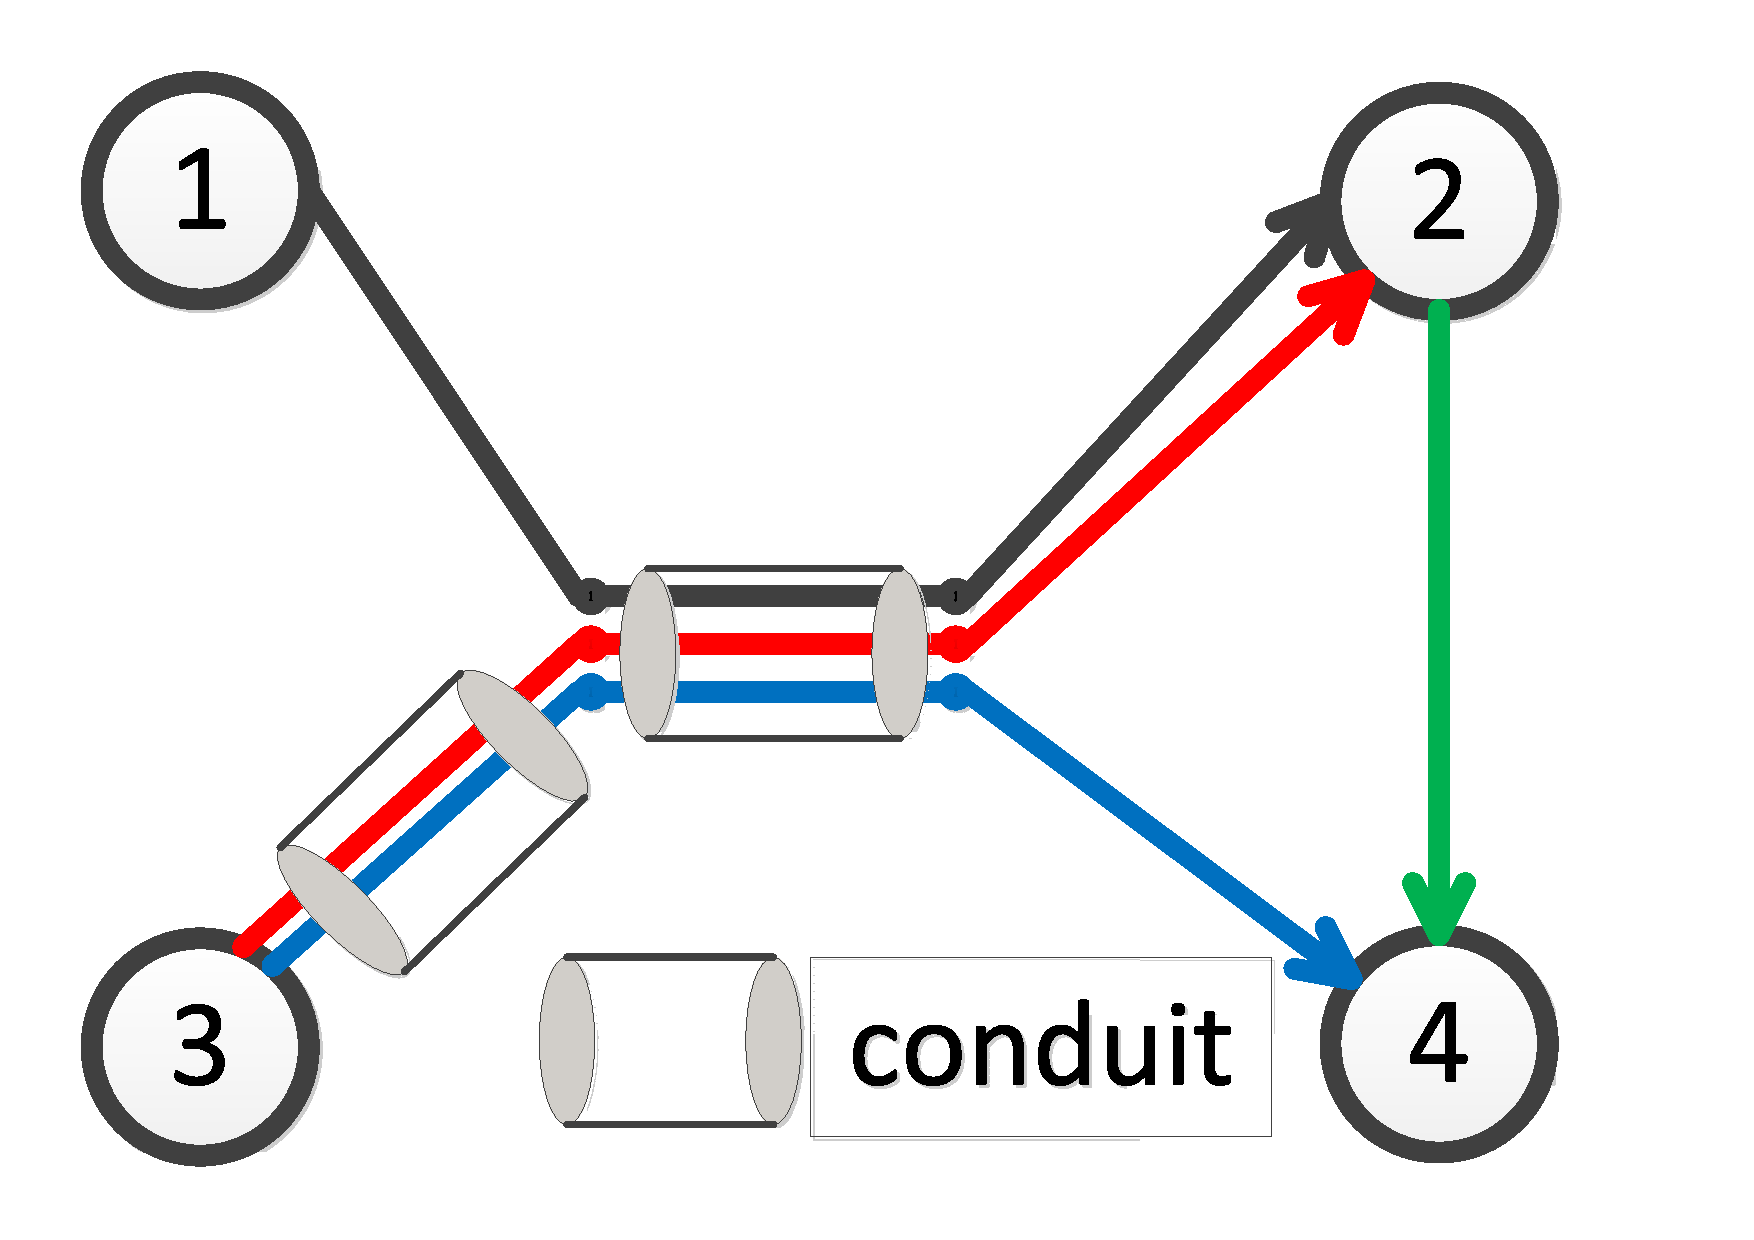
\includegraphics[width=2.2 in]{figures/PhysicalGraph}
}
\subfigure[逻辑网络]{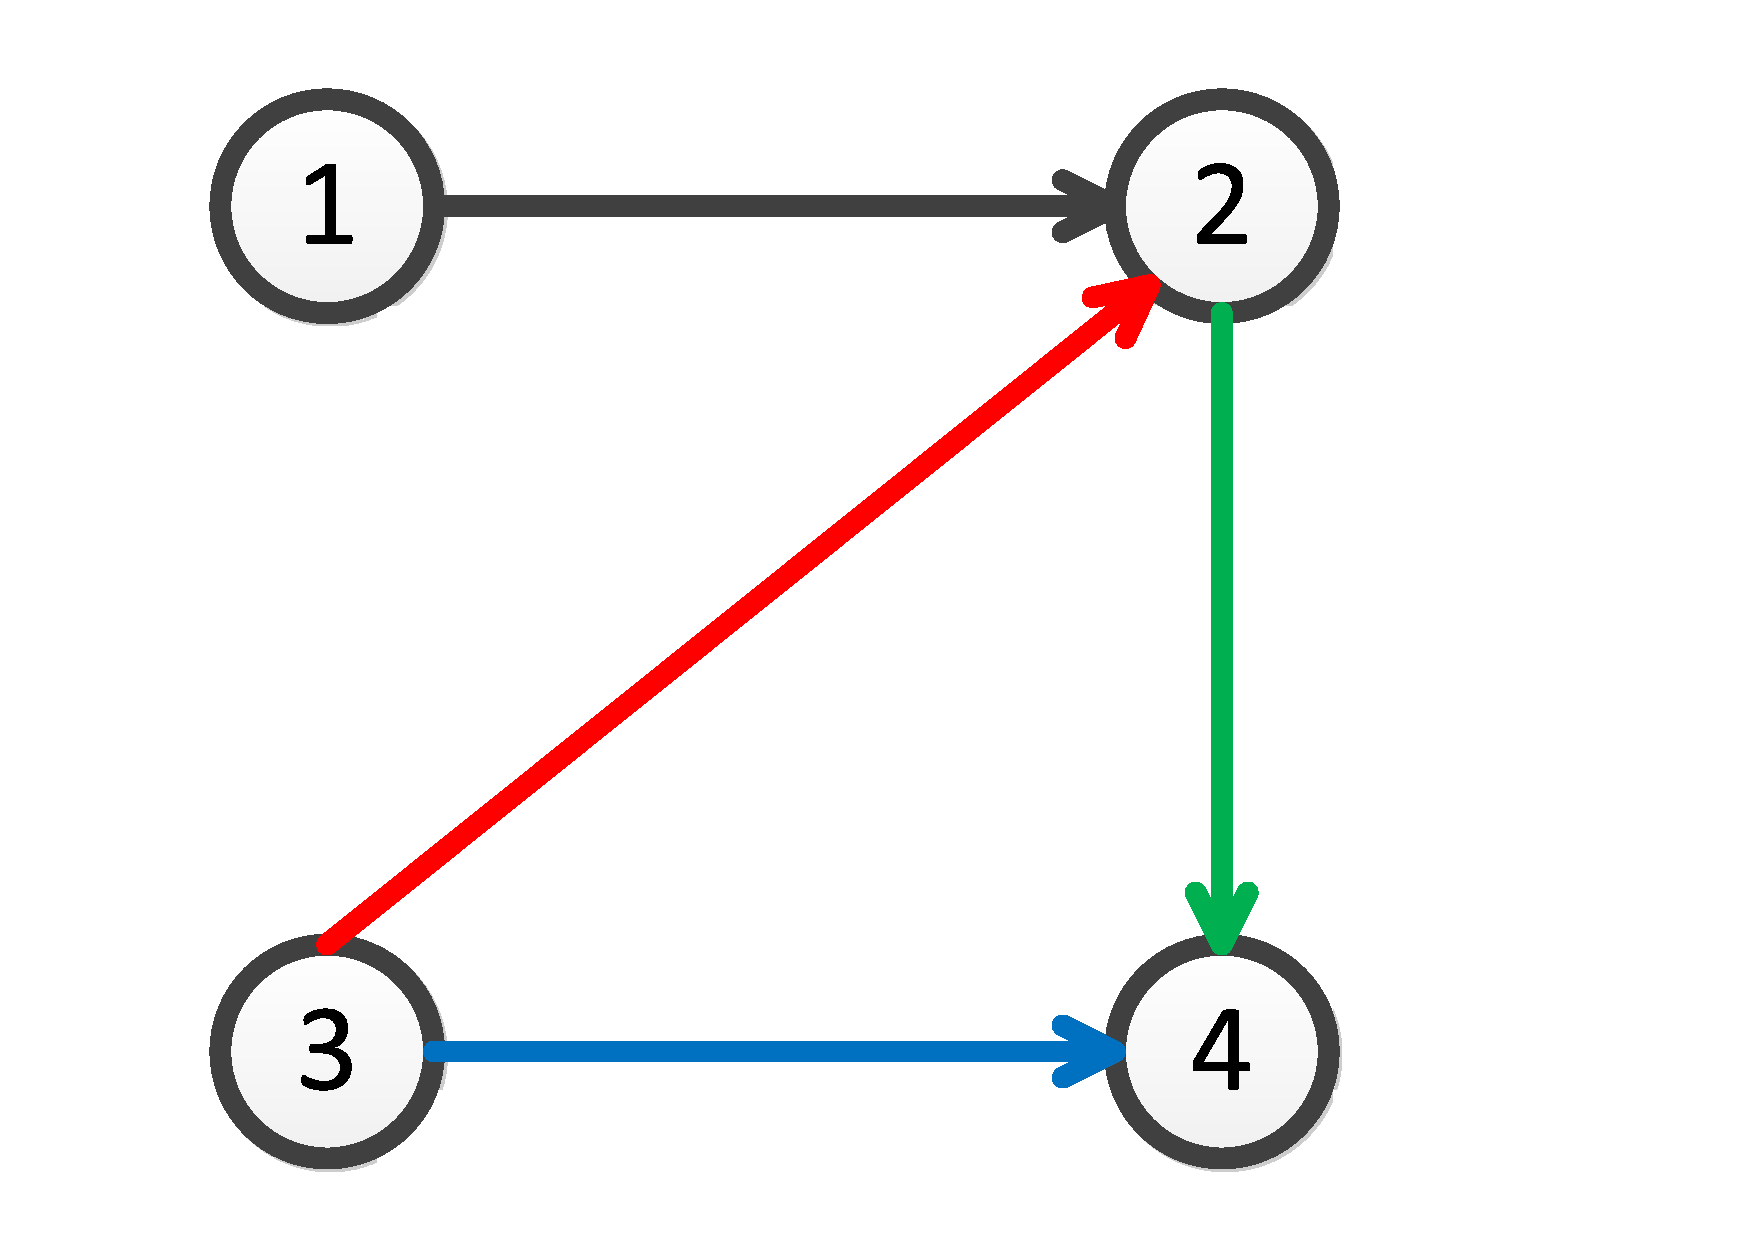
\includegraphics[width=1.8 in]{figures/VirtualGraph}
}
\caption{共享风险链路组(SRLG)实例}\label{fig:SRLGgraph}
\label{fig:Logic shift operation}
\end{figure}

设$\mathbb{R}$为网络中的风险集(故障)。每个风险可能对应于导管断开、光纤断裂、在一个节点上的驱动故障、软件故障或这些因素的任何组合。对每一个共享风险链路组$r_i \in \mathbb{R}$ 是指与其风险$r_i$ 相关的链路集合$\mathbb{R}_{r_i}$,$1\leq i\leq \chi$ 和 $\chi=|{\mathbb{R}}|$是共享风险链路组集合的个数。如图\ref{fig:CompositeGraph}(a) 所示,该图包含五个共享风险链路组集合$\mathbb{R}_{r_1}=\{e_1,e_9\}$, $\mathbb{R}_{r_2}=\{e_2,e_3,e_{19}\}$, $\mathbb{R}_{r_3}=\{e_2,e_4,e_{11},e_{17}\}$, $\mathbb{R}_{r_4}=\{e_5,e_{13}\}$, $\mathbb{R}_{r_5}=\{e_{15},e_{18}\}$。 在这个例子中,链路$e_2$同属两个共享风险链路组集合里$\mathbb{R}_{r_2}$ 和 $\mathbb{R}_{r_3}$。

SRLG不相交路径在它们之间没有任何共同的风险资源,也就是说,由于风险而导致的路径失败不会影响其他路径。图\ref{fig:CompositeGraph}(b)显示两条SRLG 不相交路径对,表示为AP 和BP。因为这两条路径没有共同的风险资源,如果AP 失败,BP仍然可以工作。本章主要讨论了两条不相交的路径,即可以描述如下。

\textbf{Min-Min SRLG完全不相交(分离)路径对问题}。给定一个图$G(V,E)$,每条链路$e_i\in \mathbb{E}$ 相关联一个权重$w_{e_i}$,一个源节点$s$和一个目的节点$d$,找到一对从$s$ 到$d$ 的SRLG不相交路径对(表示为AP和BP),而且要求这两条不相交路径中路径权重较小的那条路径权重最小化,形式化如下:

\begin{equation}
\begin{array}{*{20}{c}}
   {\mathop {minimize}\limits_{AP,BP} } & {\min \left( {{w_{AP}},{w_{BP}}} \right)}  \\
   {subject\ to} & {{r_{AP}} \cap {r_{BP}}{\rm{ = }}\phi }  \\
   {} & {\mathbb{AP} \cap \mathbb{BP}{\rm{ = }}\phi }  \\
\end{array}
\label{eq:problem definition}
\end{equation}

即${w_{AP}}$ 和 ${w_{BP}}$是AP和BP的路径权重,$\mathbb{AP}$ 和 $\mathbb{BP}$分别是路径AP和BP 上的链路集,${r_{AP}}$ 和 ${r_{BP}}$分别是影响路径AP和BP的SRLG 集。

\begin{figure*}[htbp]
  \centering
  % Requires \usepackage{graphicx}
  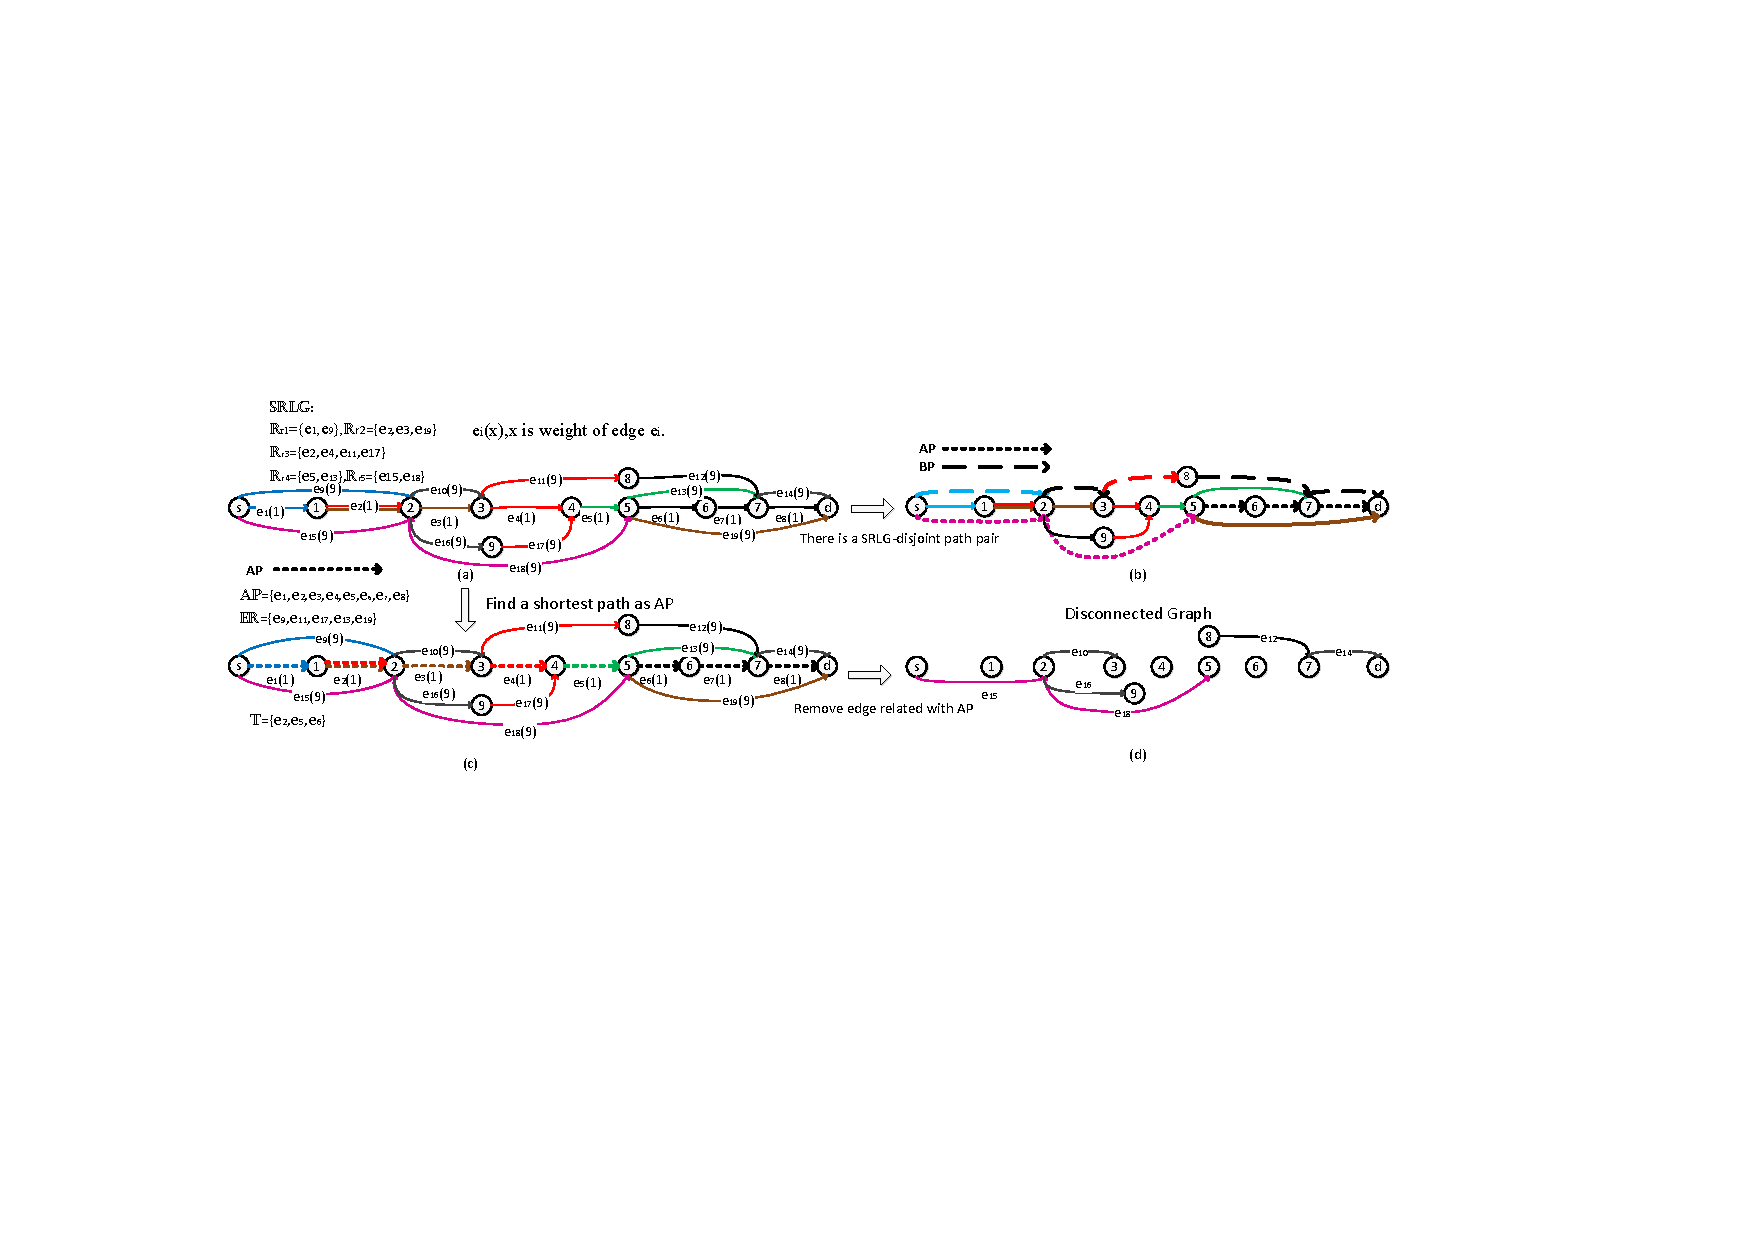
\includegraphics[width=7.2in]{figures/CompositeGraph}
  \caption{SRLG不相交路径对实例}
  \label{fig:CompositeGraph}
\end{figure*}

\subsection{问题的线性规划方程}
首先介绍线性规划方程有关的一些必要的定义:
\begin{enumerate}
  \item 零列向量:$\textbf{0}=[0,0,\ldots,0]^T$
  \item 单位列向量:$\textbf{1}=[1,1,\ldots,1]^T$
  \item 边权重的行向量:$w=[w_e]_{e\in \mathbb{E}}$,其中边的权重$w_e$($e\in \mathbb{E}$)
  \item 源目标列向量:$u=[u_v]^T_{v\in \mathbb{V}}$,其中${\rm{u_v}} = \left\{ {\begin{array}{*{20}{c}} 1&{if\ v = s}\\{ - 1}&{if\ v = d}\\ 0&{otherwise} \end{array}} \right.$
  \item 节点边关联矩阵:$A=[a_{v,e}]_{\mathbb{V}\times \mathbb{E}}$ 其中 \\ ${\rm{a_{v,e}}} = \left\{ {\begin{array}{*{20}{c}} 1&{if\ edge\ e\ originates\ from\ node\ v}\\ { - 1}&{if\ edge\ e\ terminates\ at\ node\ v}\\ 0&{otherwise}
\end{array}} \right.$
  \item 风险边关联矩阵:$H=[h_{r,e}]_{R\times E}$,其中${\rm{h_{r,e}}} = \left\{ {\begin{array}{*{20}{c}} 1&{if\ edge\ e \in \mathbb{R}_r}\\ 0&{otherwise} \end{array}} \right.$
  \item  边决策变量的列向量 包含在路径$i=AP,BP$:$x_i=[x_{i,e}]^T_{e\in \mathbb{E}}$ , 其中\\${x_{i,e}} = \left\{ {\begin{array}{*{20}{c}} 1&{if\ edge\ e \in path\ p_i}\\0&{otherwise}\end{array}} \right.$
\end{enumerate}

从s到d的两条SRLG不相交路径最小路径权重最小化的问题,整数线性规划ILP方程表示如下:

\begin{equation}
\begin{array}{*{20}{c}}
   {\mathop {minimize}\limits_{AP,BP} } & {\min \left( {{\sum\limits_{e\in \mathbb{E}}w_e*x_{AP,e}},{\sum\limits_{e\in \mathbb{E}}w_e*x_{BP,e}}} \right)}\\
   {subject\ to} & A\times x_i=u,(i=AP,BP) \\
   {} & x_{AP}+x_{BP}\leq \textbf{1}\\
   {} & (h_{r}\times x_{AP}^T)+h_{r}\times x_{BP}^T \leq \textbf{1}(1\leq r \leq \mathbb{R})
\end{array}
\label{eq:problem definition}
\end{equation}



从s到d的两条SRLG不相交路径最小路径权重最小化的问题,整数二次规划方程IQCP 表示如下:

\begin{equation}
\begin{array}{*{20}{c}}
   {\mathop {minimize}\limits_{AP,BP} } & {\min \left( {{\sum\limits_{e\in \mathbb{E}}w_e*x_{AP,e}},{\sum\limits_{e\in \mathbb{E}}w_e*x_{BP,e}}} \right)}  \\
   {subject\ to} & A\times x_i=u,(i=AP,BP) \\
   {} & x_{AP}+x_{BP}\leq \textbf{1}\\
   {} & H\times x_{AP}\times x_{BP}^T\times H^T = \textbf{0}\\
\end{array}
\label{eq:problem definition}
\end{equation}

约束$A\times x_i=u,(i=AP,BP)$保证了基于$x_i$选择的边组成一条从s到d的路径。

约束$x_{AP}+x_{BP}\leq \textbf{1}$保证这两条路径是边不相交的。

约束$(h_{r}\times x_{AP}^T)+h_{r}\times x_{BP}^T \leq \textbf{1}$和$H\times x_{AP}\times x_{BP}^T\times H^T = \textbf{0}$保证这两条路径是SRLG不相交的。

\subsection{复杂度规模}
\begin{theorem}
\label{le:lemma1}
    Min-Min SRLG-不相交路径对问题复杂度是 NP-complete.
\end{theorem}
\begin{proof}
Min-Min链路不相交路径对问题是NP-complete\cite{bhatia2006finding}。Min-Min链路不相交路径问题是Min-Min SRLG不相交路径问题的子问题。设
Min-Min SRLG不相交路径问题的复杂性为C(A),则NP-complete$\leq$C(A).

为了求Min-Min SRLG不相交路径问题的时间复杂度,首先假设了一个问题B(问题B的复杂度表示为C(B)),问题B定义为找到两条SRLG不相交路径并且路径较小的路径其权重小于或等于M(M 是大于零的整数)。Min-Min SRLG不相交路径问题A 与问题B等价,显而易知,M必须大于零且小于$\sum\limits_{e_i\in \mathbb{E}}w_{e_i}$。例如,假设0≤M≤10 和m=6 是最优解,通过经典的二分法(binary search method)其时间复杂度为O(log(N)),如图\ref{fig:binarySearch}所示,通过二分法得到了两条不相交路径,较小的路径其权重为m,因此问题A与 问题B等价。
\begin{figure}[htbp]
  \centering
  % Requires \usepackage{graphicx}
  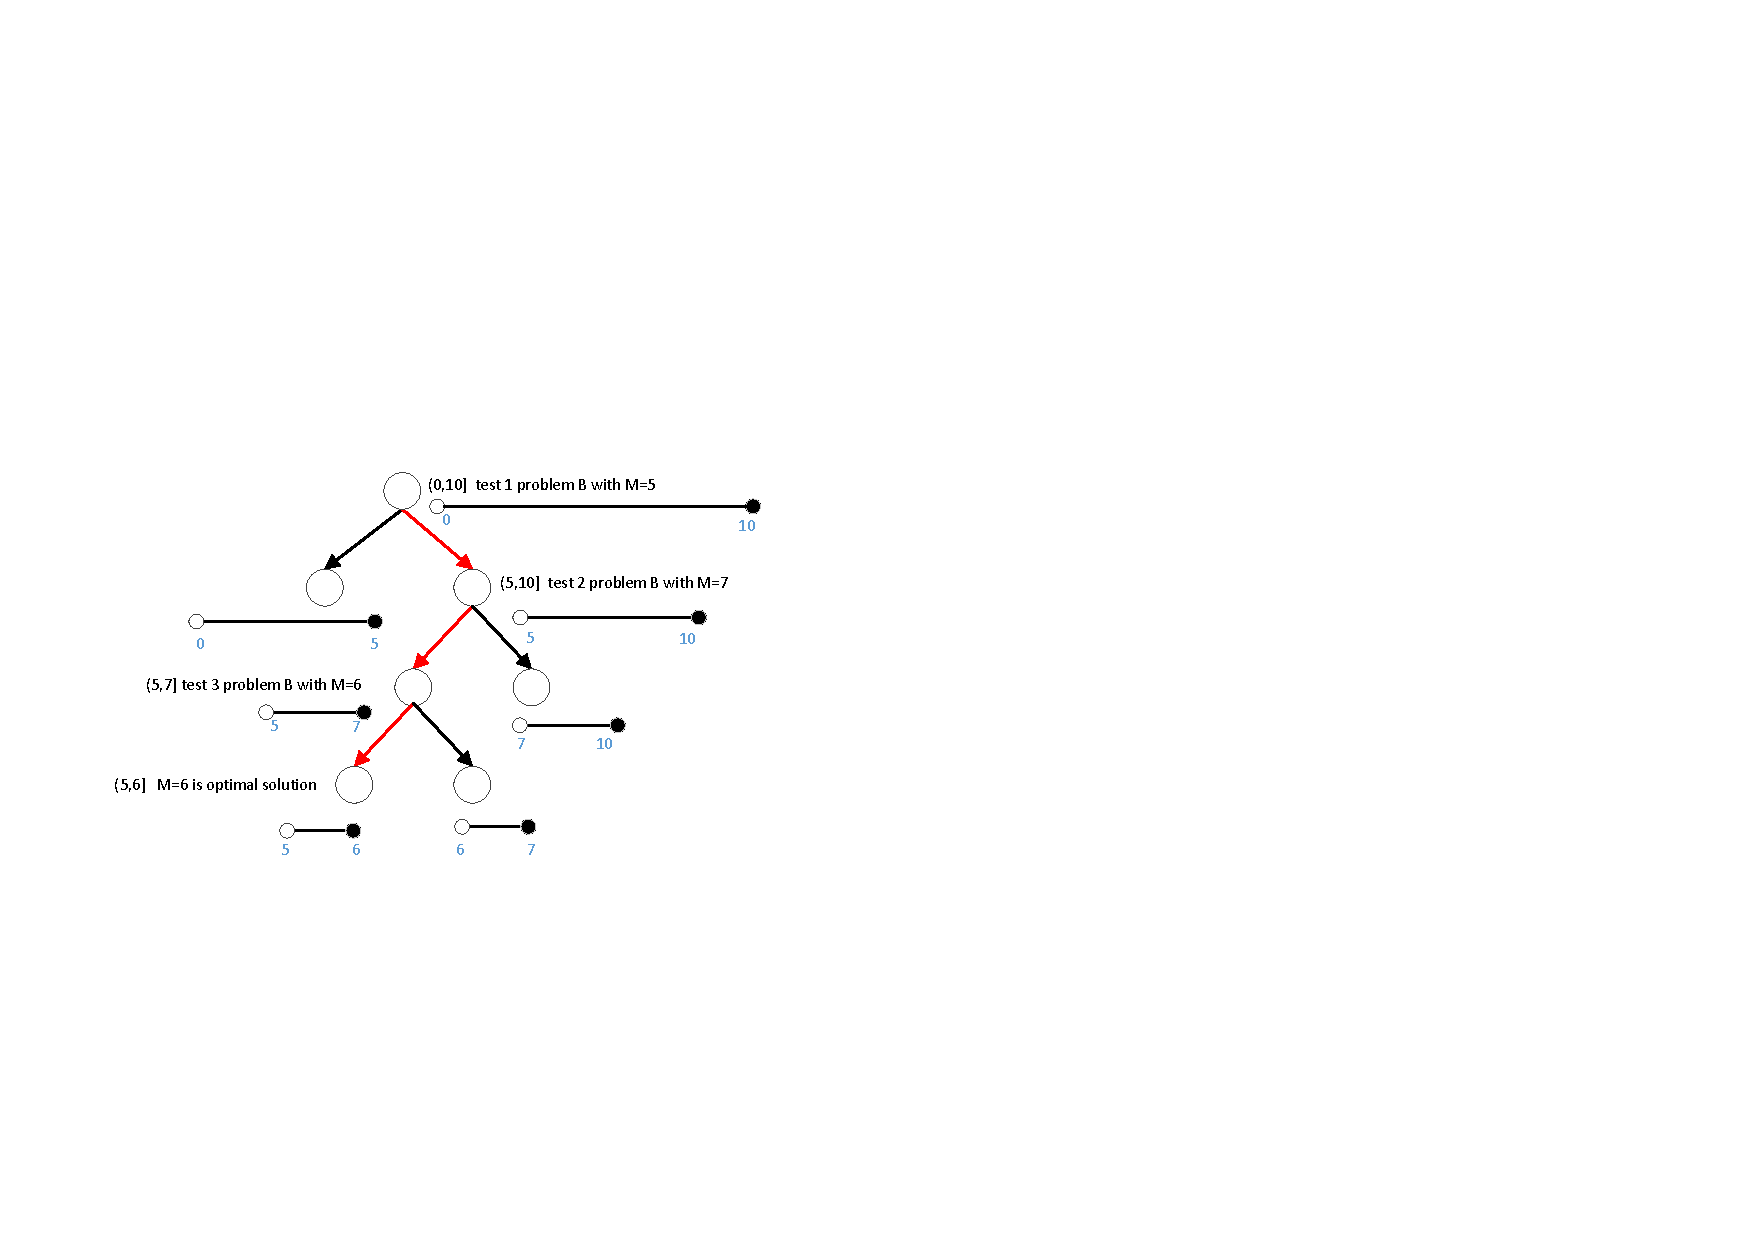
\includegraphics[width=4.0in]{figures/binarySearch}
  \caption{二分法求最优解实例}
  \label{fig:binarySearch}
\end{figure}
假设程序X在输入问题B时,如果问题B没有解,则程序Y立即停止,否则程序B继续执行并获得问题B的解,因此问题B 可以归约为NP-hard问题。因此C(B)$\leq$NP-hard。

此外,给定任意两条路径,很容易在多项式时间内判别这两条路径是否为SRLG 不相交路径,较小的路径其权重小于或等于M,从而使得C(B)$\leq$NP-complete。 当B的复杂度等于A时,有C(A)=C(B)$\leq$NP-complete。因此,A=NP-complete。
\end{proof}
\section{原有算法概述}

为了解决SRLG不相交路径问题,一种可能的方法是0-1整数线性规划(ILP)\cite{hu2003diverse},通过分支限界法(branch-and-bound)来搜索选择最优的主路径和备份路径。该方法时间复杂度高,不适用于大型网络。为了降低算法的复杂度,基于APF的启发式算法\mycite{oki2002disjoint,li2002fiber,eppstein1998finding}能够求Min-Min SRLG 不相交路径问题的近似最优解。首先使用Dijkstra算法(或任何其他最短路径算法)求出主路径,求主路径时不考虑其相应的备用路径情况,在删除AP沿线的链路并且与AP共风险的节点和链路后,再利用最短路算法求的备用路径。

然而,使用APF启发式算法的有一个主要缺陷,一旦求得路径AP后也可能无法找到相对的SRLG不相交路径BP,即使网络中确实存在一对不相交路径。这就是所谓的“陷阱”问题,在节\ref{sec:trapproblem} 将详细介绍陷阱问题产生的原因,即使稠密网络\cite{laborczi2001solving}中这也是可能发生,在一个稀疏连接的网络中当然是不能被忽略。陷阱问题分为两种:不可避免的陷阱和可避免的陷阱。不可避免的陷阱是受拓扑约束的,任何算法都无法解决。如果网络不是2-边连通度的,则没有算法可以保证在拓扑中存在两个SRLG不相交路径。另一方面,当两个节点之间存在SRLG不相交路径对,但由于路由算法的缺陷而找不到时,就会出现一个可避免的陷阱,在本章中只考虑了可避免的陷阱。

对简单的APF算法扩展,提出了K-最短路径(KSP)算法来处理节点/链路不相交路径的陷阱问题。虽然它是处理陷阱问题最有效的算法之一,但它在大型网络中的性能受到影响,因为KSP 可能会涉及多路径搜索测试,直到它找到不相交路径。当前候选的路径AP遇到陷阱问题后,仅根据路径长度选择下一个要测试的候选AP,而不考虑当前候选AP 的那条链路(或那些链路)导致查找不相交路径BP 失败。因此,为了找到一对不相交路径对,需要对大量的路径进行测试,这就引入了KSP算法中与K 相关的时间复杂度。对于遇到陷阱问题的AP,应用从AP 路径导出的SRLG冲突链路集来指导将来的AP路径测试。这在很大程度上有助于减少寻找替代路径的时间复杂度。

其它的SRLG不相交路径算法,搜索最大SRLG不相交路径对,并且路径间共享最小数目的公共链路。由于AP 和BP 可能具有相同的风险资源组,通过这种方法找到的解决方案是不可靠的。我提出的算法目标是寻找SRLG完全不相交路径对。Xu\cite{xu2003trap}试图找到SRLG完全不相交路径。但他的算法减少了问题的搜索空间,加快了路径搜索的速度。然而,它可能会以较大的代价返回路径,因为在削减后的搜索空间可能会失去最优解。相反,为了大大加快搜索过程,利用SRLG冲突链路集将原问题划分为多个子问题,这些子问题可以并行执行。因此,提出的算法可以运行得更快,返回主路径成本非常低。

Datta\cite{datta2008graph}提出方法是将SRLG不相交路径问题转化为链路不相交路径问题,然后利用链路不相交路径算法来解决。然而,只有特殊的SRLG 星型模式可以转换为链路不相交,这样就限制了该算法的广泛应用。当AP遇到陷阱问题时,CoSE\cite{rostami2007cose}算法试图找到一个SRLG集合,任何AP 路径包含了这个SRLG集合里的所有SRLG,则必定找不到任何的与其对应的SRLG不相交路径BP。CoSE 首先通过多轮搜索查找多个AP共享的SRLG,并且组成一个SRLG集合,然后根据SRLG 集合来划分原始问题以搜索SRLG不相交路径对。而不使用SRLG 中链路之间共享风险的特性,CoSE方法的这种穷尽搜索需要非常高的计算开销。



\section{陷阱问题}
\label{sec:trapproblem}
基于APF的启发式算法可能会陷入“陷阱”问题。也就是说,当一个AP被确定时,即使网络中确实存在一对不相交路径对,它也可能无法找到SRLG不相交的BP路径。图\ref{fig:CompositeGraph}(c),(d)说明了陷阱问题,虚线表示一条AP 路径,其链路集为$\mathbb{AP}=\{e_1,e_2,e_3$ $,e_4,e_5,e_6,e_7,e_8\}$,在删除AP上的链路和与AP 共享风险的链路后,图\ref{fig:CompositeGraph}.(d) 所示的不存在从s到d的路径,因此找不到相对应的BP。

虽然KSP算法被认为是解决陷阱问题的有效算法,但它可能面临着效率低下的问题。如图\ref{fig:KSPproblem}所示假设$e_1, e_2, e_3, e_4$的链路权重比其他链路大得多。此外,在$e_1, e_2, e_3, e_4$中,$e_1$ 和$e_2$ 的链路权重远小于$e_3$,$e_4$。然后,在KSP算法多次找从s到d的K 短路时,总是包含$e_1,e_2$ (虚线表示)。则最短AP 总会遇到陷阱问题,因为$e_1$和$e_4$ 具有相同的风险,因此无法找到BP。为了避免陷阱问题,必须将K设为一个大值,这给KSP带来了很高的时间复杂度。
\begin{figure}[htbp]
\centering
% Requires \usepackage{graphicx}
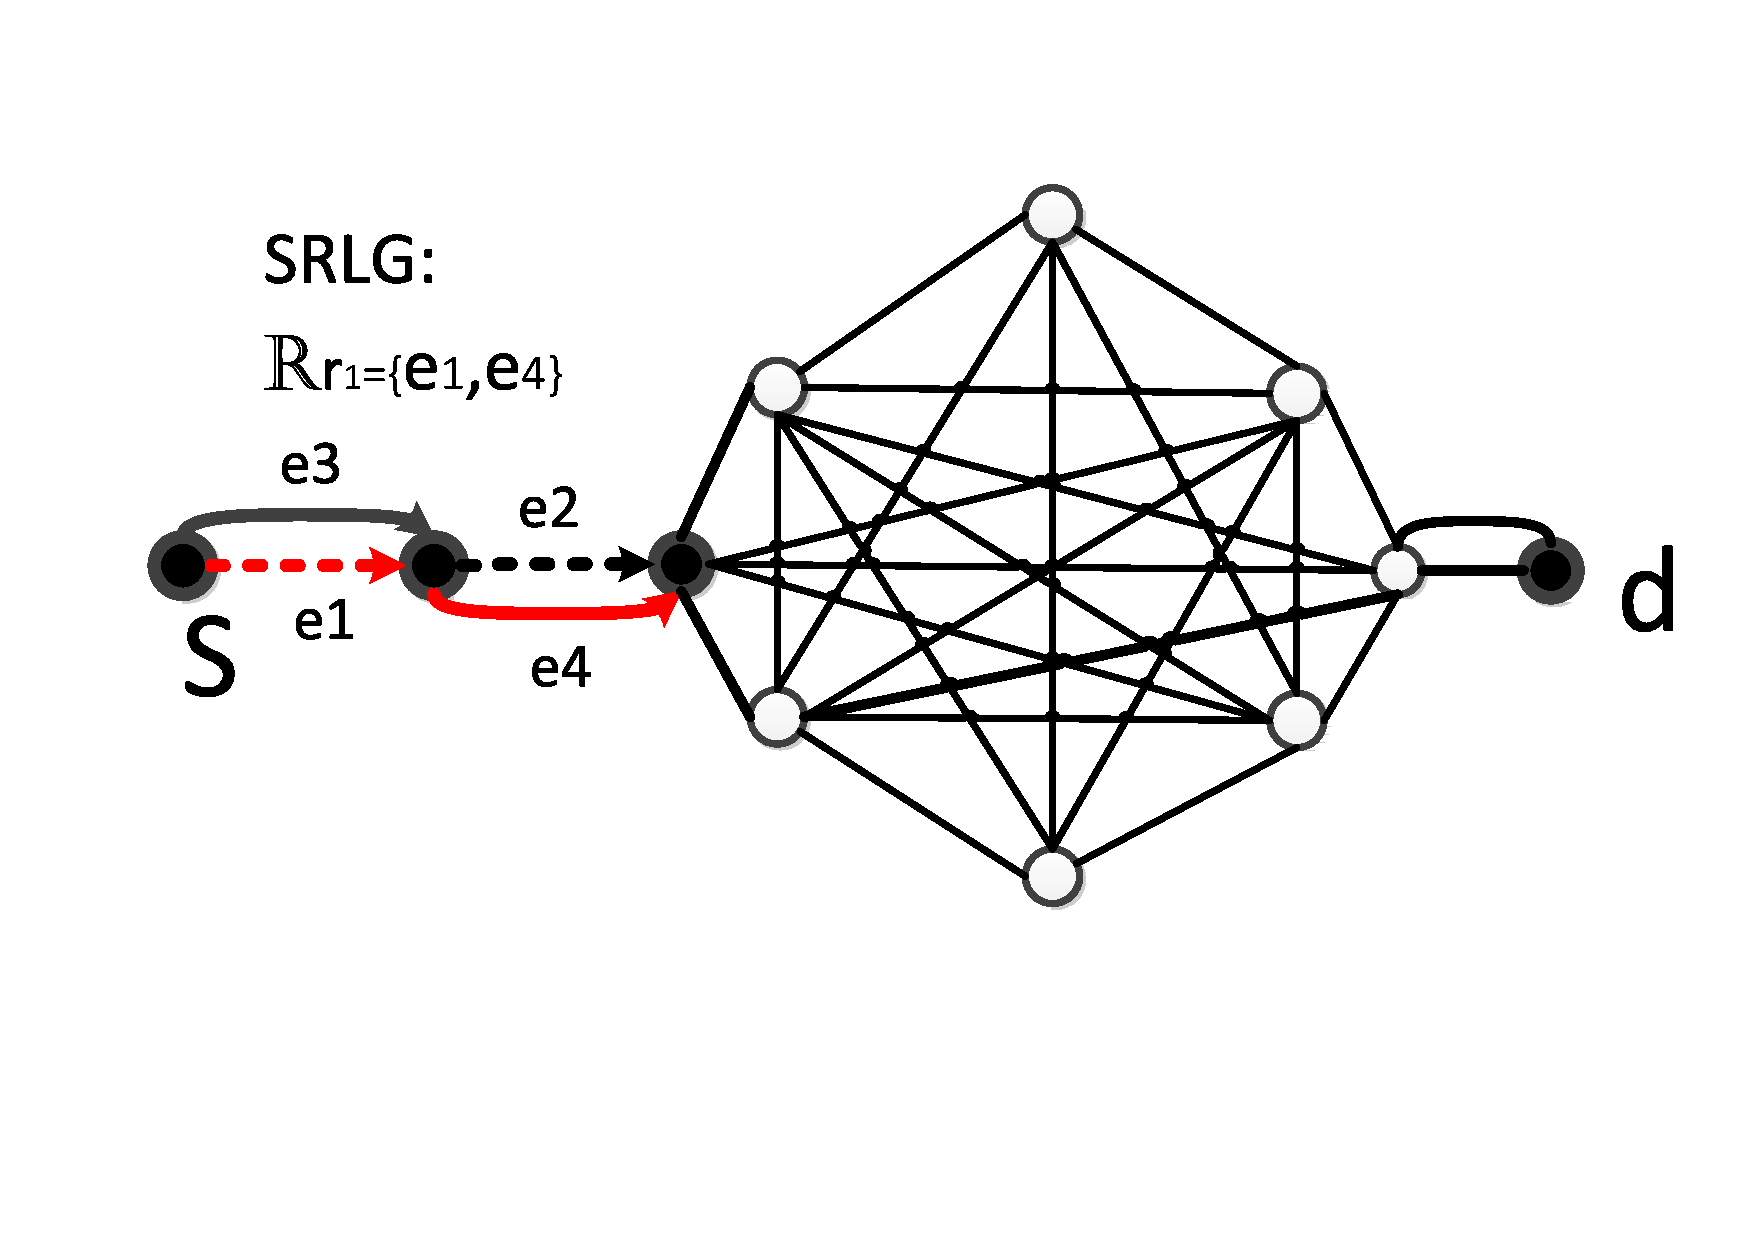
\includegraphics[width=4.0in]{figures/KSPproblem}
  \caption{演示KSP算法时间效率低的实例}
  \label{fig:KSPproblem}
\end{figure}


\section{分而治之的快速SRLG完全不相交路径对算法}
当一个陷阱问题发生,并且对于给定的AP没有SRLG不相交路径BP时,AP中可能存在一个子链路集,这样任何通过这个链路集里所有的这些“问题”链路的AP都不能找到一条相对应SRLG不相交BP路径,称之为\textbf{SRLG冲突链路集}。与KSP 不同,当最短AP路径遇到陷阱问题时,将通过两个主要步骤来解决这个问题。如图\ref{fig:KSPproblem} 所示的例子中,将首先找到图\ref{fig:KSPproblem} 中的SRLG冲突链路集合,然后应用分而治之算法将原问题划分为两个子问题$\mathcal{P}(\emptyset,\{e_1\})$和 $\mathcal{P}(\{e_1\},\{e_2\})$。 这两个子问题可以在多核CPU平台上并行执行,快速得到SRLG不相交路径对。
\subsection{分而治之}
在得到SRLG冲突链路集后,设计了一种分而治之的算法,将原Min-Min SRLG不相交路径问题划分为多个子问题,并行执行,加快求SRLG不相交路径对的过程。

为了便于问题划分,首先定义了两个不相交的链路集合$\mathbb{I}$和$\mathbb{O}$,其中称$\mathbb{I}$为包含集集合,$\mathbb{O}$称为排除集集合。由$\mathcal{P}({\mathbb{I},\mathbb{O}})$表示的Min-Min SRLG不相交问题,用于寻找一对AP和BP,其中AP是所有可能的AP中最短的,其中路径$AP$必须经过$\mathbb{I}$集合里的所有链路和不经过$\mathbb{O}$集合里的所有链路。

最初,让$\mathbb{I}=\emptyset$ ${\mathbb{O}}=\emptyset$,原来的Min-Min SRLG不相交路径对问题可以用$\mathcal{P}(\emptyset,\emptyset)$ 表示。给定SRLG冲突链路集$\mathbb{T}=\{{e_1},{e_2}, \cdots ,{e_{\left| \mathbb{T} \right|}}\}$,原问题$\mathcal{P}(\emptyset,\emptyset)$可按以下步骤划分。

\begin{enumerate}
  \item 首先,$\mathcal{P}(\emptyset,\emptyset)$能被划分成两个子问题$\mathcal{P}(\emptyset,\{e_1\})$ 和 $\mathcal{P}(\{e_1\},\emptyset)$。
  \item 类似,$\mathcal{P}(\emptyset,\{e_1\})$能被划分成两个子问题 $\mathcal{P}(\{e_1,e_2\},\emptyset)$ 和 $\mathcal{P}(\{e_1\},\{e_2\})$。
  \item 这个划分步骤持续直到步骤$|\mathbb{T}|$,问题$\mathcal{P}(\{e_1,e_2,\cdots ,{e_{\left| \mathbb{T} \right|-1}}\},\emptyset)$ 进一步的拆分成两个子问题$\mathcal{P}(\{e_1,e_2,\cdots ,{e_{\left| \mathbb{T} \right|-1}}, {e_{\left| \mathbb{T} \right|}}\},\emptyset)$ 和 $\mathcal{P}(\{e_1,e_2,\cdots ,{e_{\left| \mathbb{T} \right|-1}}\},{e_{\left| \mathbb{T} \right|}})$。注意到,子问题$\mathcal{P}(\{e_1,e_2,\cdots ,{e_{\left| \mathbb{T} \right|-1}}, {e_{\left| \mathbb{T} \right|}}\},\emptyset)$是无解的。
\end{enumerate}



除了子问题$\mathcal{P}(\{e_1,e_2,\cdots ,{e_{\left| \mathbb{T} \right|}}\},\emptyset)$外,将试图求其它每个子问题的最优解。然后选择最好的路径对(即主路径最短的路径对),作为原问题$\mathcal{P}(\emptyset,\emptyset)$的最终(最优)解。如果这些子问题都没有解,则可以得出原问题没有任何解,因为子问题包括了所有的可能的不相交路径对。

就时间复杂性而言,解决子问题所需的时间比原来的问题应该花费的更少。因为一条链路(来自集合$\mathbb{T}$) 将在计算AP的路径时被去除,这也确保了不同的AP 路径将被测试且是否存在一个SRLG不相交BP 路径。

当遇到陷阱问题时,提出的解决方案将划分原来的问题,并测试每个子问题以寻找到最终的解。在提出的分而治之方法中,子问题是由SRLG冲突链路集而得,而这个SRLG冲突链路集却是当AP路径遇到陷阱问题生成的。与现有的算法相比较,该算法在不考虑现有结果和问题的情况下,可以在很大程度上降低算法的计算量。对于图\ref{fig:DividedConquer}中的例子所示,SRLG冲突链路集是$\mathbb{T}=\{e_2,e_5,e_6\}$。拆分过程过程如图\ref{fig:DividedConquer} 所示。根据SRLG冲突链路集,应该测试总共3个子问题${{\mathcal{P}}(\{ e_2,e_5\} ,\{ e_6\} )}$, ${{\mathcal{P}}(\{ e_2\} ,\{ e_5\} )}$ 和 ${{\mathcal{P}}(\emptyset ,\{ e_2\} )}$,其中选择AP 路径权重最低的最优子问题作为原问题$\mathcal{P}(\emptyset,\emptyset)$最终的(最优)解。

注意,不需要解决子问题${{\mathcal{P}}(\{ e_2,e_5\}, \emptyset)}$ 和 ${{\mathcal{P}}(\{ e_2\},\emptyset )}$,因为它们的解已经包含在其它的子问题中。第一个解空间由两个子问题${{\mathcal P}(\{ e_2,e_5,e_6\} ,\emptyset )}$ 和 ${{\mathcal P}(\{ e_2,e_5\} ,\{ e_6\} )}$ 组成。由于SRLG冲突链路集为$\mathbb{T}=\{e_2,e_5,e_6\}$,显然,子问题${{\mathcal P}(\{ e_2,e_5,e_6\} ,\emptyset )}$是没有解的。因此,${{\mathcal P}(\{ e_2,e_5\} ,\{ e_6\} )}$的解空间等于${{\mathcal{P}}(\{ e_2, e_5\}, \emptyset)}$的解空间。同样,${{\mathcal{P}}(\{ e_2\},\emptyset )}$的解空间包括${{\mathcal{P}}(\{ e_2\} \{ e_5\}, \emptyset)}$  和 ${{\mathcal{P}}(\{ e_2\} ,\{ e_5\} )}$的解空间。
\begin{figure}[htbp]
\large{
\begin{equation*}
{\mathcal P}(\emptyset ,\emptyset )\left\{ {\begin{array}{*{20}{l}}
{{\mathcal P}(\{ e_2\} ,\emptyset )\left\{ {\begin{array}{*{20}{l}}
{{\mathcal P}(\{ e_2,e_5\} ,\emptyset )\left\{ {\begin{array}{*{20}{l}}
{{\mathcal P}(\{ e_2,e_5,e_6\} ,\emptyset )}\\
{\boxed{{\mathcal P}(\{ e_2,e_5\} ,\{ e_6\} )}}
\end{array}} \right.}\\
{\boxed{{\mathcal P}(\{ e_2\} ,\{ e_5\} )}}
\end{array}} \right.}\\
{\boxed{{\mathcal P}(\emptyset ,\{ e_2\} )}}
\end{array}} \right.
\end{equation*}
}
\caption{分而治之的解决方案}
\label{fig:DividedConquer}
\end{figure}




\subsection{SRLG冲突链路集合}
在本节中,我将描述了如何找到一个SRLG冲突链路集合,当在网络$G$中给定一个AP 路径并且没有SRLG 不相交的BP路径。
\subsubsection{边容量设置准则}
如\ref{subsubsec:maxFlow}节介绍的,如果在图G中去除所有在边割集$\mathbb{\mathbb{L}}_{\Phi}$ 的所有边,则$|f| = 0$。也就是说,不存在任何流能从$s$到$d$。在本文中,试图基于割集的概念找到SRLG冲突链路集合。如果AP从s到d流通,经过的链路与割集$\mathbb{\mathbb{L}}_{\Phi}$ 共享风险,则找不到任何与其对应的SRLG不相交路径BP,因为没有一条在割集中的链路可以被BP 选择。

基于割集基础为了找到SRLG 冲突链路集,构造了一个新图$G^*$ ,如下所示。
\begin{enumerate}
  \item $G^*$与$G$的节点和链路拓扑关系一样。
  \item 跟每条链路$e_i$相关的链路权重$w_{e_i}$是跟其相对应图$G$中边的权重一样的。
  \item 使用公式\ref{eq:capacity principle}的准则设置每条边$e_i \in \mathbb{E}$相关的容量$c_{e_i}$。
\end{enumerate}
\begin{equation}
c_{e_i} = \left\{ {\begin{array}{*{20}{c}}
   1 & {e_i{\rm{ }} \in {\rm{ \mathbb{AP}}}}  \\
   {\left| \mathbb{AP} \right|+1} & {e_i{\rm{ }} \in {\rm{ \mathbb{E}}}{{\rm{\mathbb{R}}}}}  \\
   {\left| {{\rm\mathbb{AP}}} \right| + \left( {\left| {{\rm\mathbb{AP}}} \right| + 1} \right)\times \left| {{\rm{\mathbb{E}}}{{\rm{\mathbb{R}}}}} \right| + 1} & {otherwise}  \\
\end{array}} \right.
\label{eq:capacity principle}
\end{equation}
$\mathbb{AP}$指在图$G$中较小权重路径$AP$上所有链路的集合,和$\mathbb{\mathbb{ER}}$指不属于路径$AP$上的边但是与路径$AP$上的边共享风险的链路集合。

如图\ref{fig:CompositeGraph}(c)所示,路径$AP$的边集合$\mathbb{AP}=\{e_1,e_2,e_3,e_4$
$,e_5,e_6,e_7,e_8\}$, $\mathbb{\mathbb{ER}}=\{e_9,e_{11},e_{17},e_{13},e_{19}\}$。$|\mathbb{AP}|=8$, $|\mathbb{\mathbb{ER}}|=5$, $|\mathbb{AP}|+1=9$ 和 ${\left| {{\rm{\mathbb{AP}}}} \right| + \left( {\left| {{\rm{\mathbb{AP}}}} \right| + 1} \right)\times \left| {{\rm{\mathbb{E}}}{{\rm{\mathbb{R}}}}} \right| + 1}=54$。产生一个新图$G^*$如图\ref{fig:FlowStarGraph}所示,在图$G^*$中边的容量是根据公式(\ref{eq:capacity principle})所设置。

$r_P$表示影响路径$P$上的风险集合,即$r_P=\{r\in \mathbb{R}$: 路径 $P$ 包含的链路在 $\mathbb{R}_r$ 中$\}$。 如图\ref{fig:CompositeGraph}(c) 所示,在路径$AP$ 上的边集$\mathbb{AP}=\{e_1,e_2,e_3,e_4,e_5,e_6,e_7,e_8\}$,并且$e_1\in \mathbb{R}_{r_1}$, $e_2\in \mathbb{R}_{r_2}$, $e_2\in \mathbb{R}_{r_3}$, $e_3\in \mathbb{R}_{r_2}$, $e_4\in \mathbb{R}_{r_3}$, $e_5\in \mathbb{R}_{r_4}$,路径$AP$ 的风险集合是${r}_{{AP}}=\{r_1, r_2, r_3, r_4\}$。$\mathbb{\mathbb{ER}}$ 代表不属于$AP$上的链路但是与$AP$共享相同的风险集合的链路。如图\ref{fig:CompositeGraph}(c) 所示,$\mathbb{\mathbb{ER}}=\{e_9,e_{11},e_{17},e_{13},e_{19}\}$。

\begin{figure}[tp]
  \centering
  % Requires \usepackage{graphicx}
  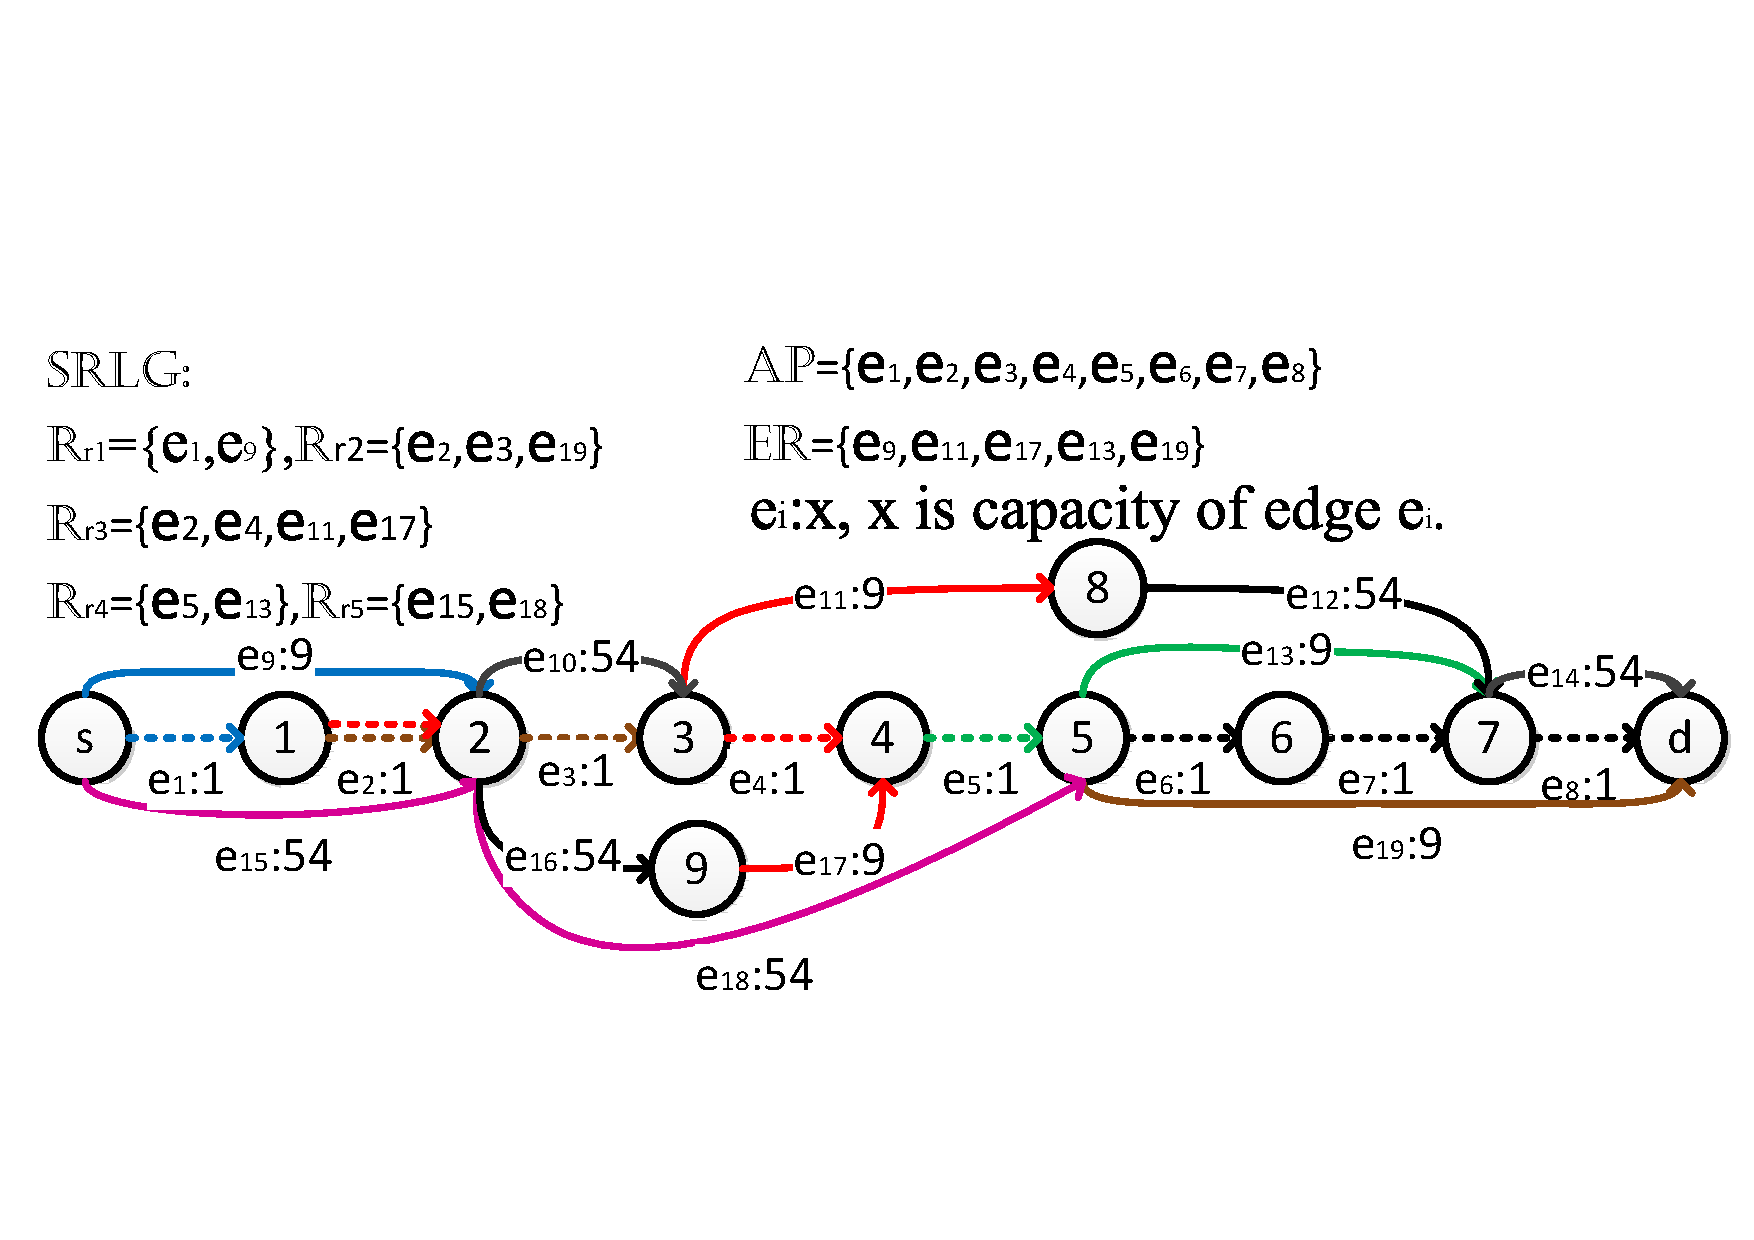
\includegraphics[width=4.5in]{figures/FlowStarGraph}
  \caption{图$G^*$实例}\label{fig:FlowStarGraph}
\end{figure}



\subsubsection{最小割最大流定理}
\label{subsubsec:maxFlow}
设$G=(\mathbb{\mathbb{V}},\mathbb{\mathbb{E}})$是一个网络(其中$\mathbb{\mathbb{V}}$是$|\mathbb{\mathbb{V}}|$个节点的集合,$\mathbb{\mathbb{E}}$是$|\mathbb{\mathbb{E}}|$条链路的集合),其中$s\in \mathbb{V}$和$d\in \mathbb{V}$分别指源节点和终节点。链路$e_i$ 的\textbf{容量}表示该条链路的最大流量。链路的流$f_{e_i}$应该满足以下两个限制:
\begin{enumerate}
  \item 容量限制: $\forall e_i\in \mathbb{\mathbb{E}}$: $f_{e_i}\leq c_{e_i}$.
  \item 流量守恒: $\forall u\in \mathbb{\mathbb{V}}-\{s,d\}$: $\sum\limits_{v\in \mathbb{V}}f_{(v,u)}=\sum\limits_{v\in \mathbb{V}}f_{(u,v)}$,  $(v,u)$ 和 $(u,v)$ 代表链路 $e(v,u)$ 和 $e(u,v)$.
\end{enumerate}

流的值定义为$|f|=\sum\limits_{v\in \mathbb{V}}f_{(s,v)}$,其中s是源节点。它表示从s节点到d 节点的流量。\textbf{最大流量问题}:尽可能的求从s 节点到d 节点的最大流量值$|f|$。

一个 s-d 割${\Phi}=(\mathbb{S},\mathbb{D})$ 是节点$\mathbb{V}$的划分且$s \in \mathbb{S}$ 和 $d \in \mathbb{D}$,$\Phi$ 的割集合$\mathbb{\mathbb{L}}_{\Phi}$ 是一个包含边的集合。
\begin{equation}
\mathbb{\mathbb{L}}_{\Phi}=\{(u,v)\in \mathbb{E}: u \in \mathbb{S}, v \in \mathbb{D}\}.
\end{equation}

如果在割集合$\mathbb{\mathbb{L}}_{\Phi}$中的边被去除,那么在原图中的流值$|f| = 0$。即没有流能从s 节点到d 节点。一个 s-d 割${\Phi}=(\mathbb{S},\mathbb{D})$ 的容量被定义成$c(\Phi)=\sum\limits_{e_i\in \mathbb{\mathbb{L}}_{\Phi}}c_{e_i}$。\textbf{最小s-d 割 $\Phi$ 问题},最小化$c(\Phi)$即决定点集$\mathbb{S}$ 和 $\mathbb{D}$使得s-d 割${\Phi}=(\mathbb{S},\mathbb{D})$的($c(\Phi)$) 最小化 。

\textbf{最小割最大流定理}:一个s-d流的最大值等于s-d割的最小割。如图\ref{fig:FlowNetwork}所示,在图$G$ 中的流量$|f|=f_{(s,v_1)}+f_{(s,v_2)}$。 这个割$\Phi(\mathbb{S},\mathbb{D})$ 是 $\mathbb{S}=\{s,v_1,v_2,v_4\}$ 和$\mathbb{D}=\{v_3,d\}$,它是最小的割其容量为$c(\Phi)=c_{(v_1,v_3)}+c_{(v_4,v_3)}+c_{(v_4,d)}=12+7+4=23$. 显然, $|f|=c(\Phi)$, 即s-d 最大流等于所有s-d割中最小的容量。
\begin{figure}[htbp]
  \centering
  % Requires \usepackage{graphicx}
  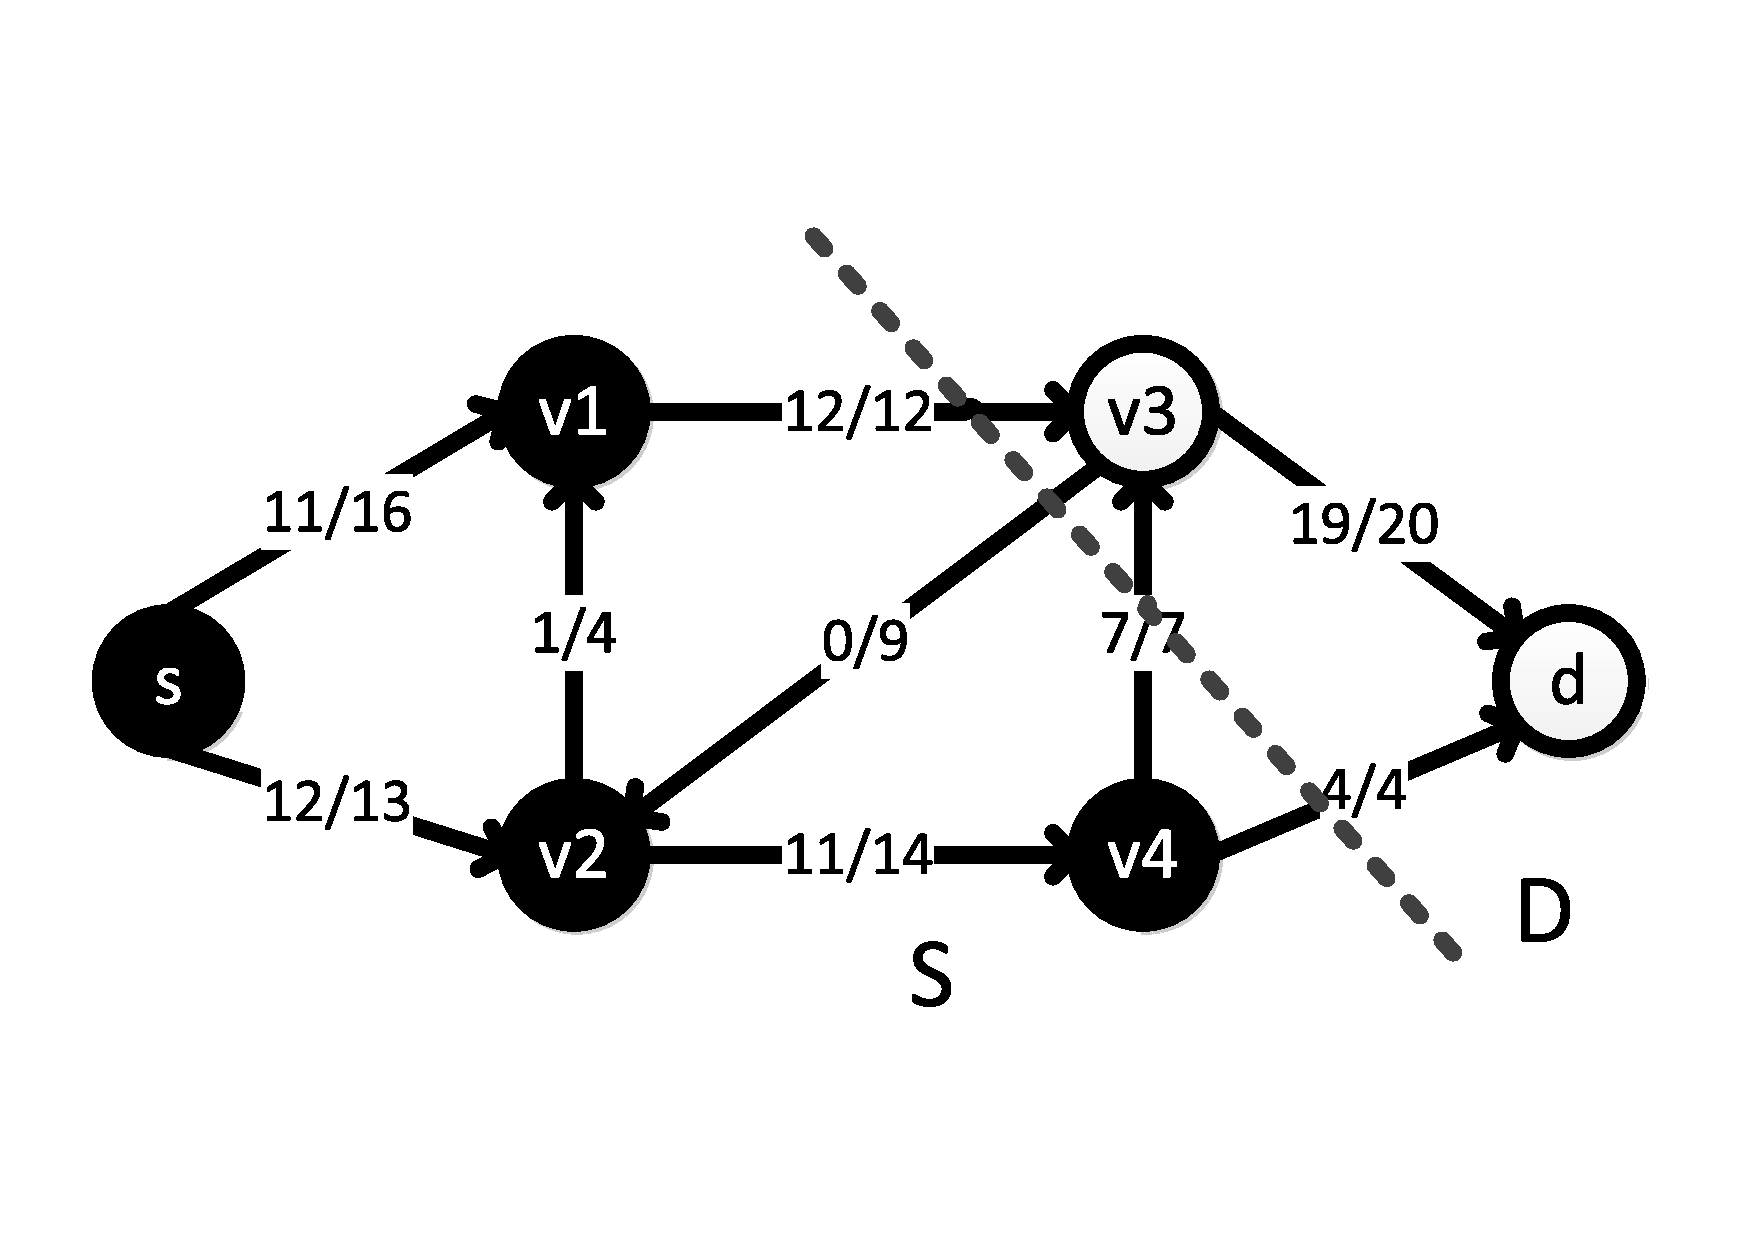
\includegraphics[width=4.0in]{figures/FlowNetwork}\\
  \caption{最大流最小割定理实例}
  \label{fig:FlowNetwork}
\end{figure}

\subsubsection{新图$G^*$中最小割集性质}
最大流最小割定理指出,在网络中,从源节点$s$到目的节点$d$的最大流值等于最小边割集的总容量,即最小的链路总容量,如果删除最小边割集上的边,将断开目的节点$d$ 与源节点$s$的连通。 提出的算法基于图的最小割集的链路集来求得最小SRLG 冲突链路集。将首先展示重建新图$G^*$的一些优良特性为求得最小SRLG冲突链路集。

\begin{lemma}
\label{le:lemma1}
    在图$G^*$中任何从$s$到$d$的路径必须经过在$\mathbb{AP}$ 或者 $\mathbb{\mathbb{ER}}$中边集合的一条边。
    %note:draw a picture to describe the proof
\end{lemma}
\begin{proof}
用矛盾法证明这条引理。假设对于某条路径AP,有另一条路径从$s$到$d$ 在图$G^*$中不与AP共享风险,即这条路径不通过$\mathbb{AP}$ 或者 $\mathbb{\mathbb{ER}}$的任何一条链路。可以很容易得出这样的结论,这条路径是与路径AP对应的SRLG不相交路径BP。这与AP 没有对应的SRLG不相交路径的说法相矛盾。
\end{proof}

\begin{lemma}
\label{le:lemma2}
    图$G^*$的任何一条最大流的流值最多为$|\mathbb{AP}|+(|\mathbb{AP}|+1)\times|\mathbb{\mathbb{ER}}|$。
\end{lemma}
\begin{proof}
假设$G^*$的最大流$f$为$|f|=k$。在$G^*$中,f可以被划分为$k$个从s到d的1 单元流。根据引理.\ref{le:lemma1},这些1-单位流中的每一个都必须通过通过$\mathbb{AP}$ 或者 $\mathbb{\mathbb{ER}}$的至少一条链路。请注意,$\mathbb{AP}$ 或者 $\mathbb{\mathbb{ER}}$ 中链路的容量分别为1或者$|\mathbb{AP}|$+1。根据$\mathbb{AP}$ 和 $\mathbb{\mathbb{ER}}$中链路的容量设置,因为$\mathbb{AP}$中的链路只能承载1-单位流量,而在ER中一条链路在$\mathbb{ER}$中能最多承载$|\mathbb{AP}|$+1单位流量。因此,最多只能有$|\mathbb{AP}|+ (|\mathbb{AP}|+1)\times|\mathbb{\mathbb{ER}}|$ 个从s到d 的单位流量。
\end{proof}

\begin{lemma}
\label{le:lemma3}
    图$G^*$最小割$\Phi$的边割集$\mathbb{L}_{\Phi}$上所有链路都在$\mathbb{AP}$ 或者$\mathbb{\mathbb{ER}}$ 中。
\end{lemma}

\begin{proof}
根据最大流最小割定理,$c(\Phi)$表示的最小切割$\Phi$的的容量,其应该等于最大流量值,根据引理 \ref{le:lemma2} 最大流量最多为$|\mathbb{AP}|+ |\mathbb{ER}|\times (|\mathbb{AP}|+1)$。 根据容量设定原则如公式\ref{eq:capacity principle}所示,一条链路既不在$\mathbb{AP}$ 也不在 $\mathbb{ER}$ ($e_i \notin \mathbb{AP}$ 和 $e_i \notin \mathbb{ER}$), 则这条链路的容量为 $c_{e_i} = \left| {{\rm\mathbb{AP}}} \right| + \left( {\left| {{\rm\mathbb{AP}}} \right| + 1} \right)\times \left| {{\rm{\mathbb{E}}}{{\rm{\mathbb{R}}}}} \right| + 1$, 这条链路是大于$|\mathbb{AP}|+(|\mathbb{AP}|+1)\times |\mathbb{ER}|$。 因此,这条链路不可能在$\mathbb{L}_{\Phi}$ 中。因此,割集$\mathbb{L}_{\Phi}$中的所有链路都必须属于边集合$\mathbb{AP}$ 或者 $\mathbb{ER}$。
\end{proof}


\begin{theorem}
    如果在图$G$中一个单元流阻塞了全部边割集$\mathbb{L}_{\Phi}$的所有边,则在原图中不会存在任何流经过这个图的割$\Phi$。
\label{th:block flow}
\end{theorem}


\begin{proof}
    如果在图$G$中一个单元流阻塞了全部边割集$\mathbb{L}_{\Phi}$的所有边,则在原图中没有流能使用边割集$\mathbb{L}_{\Phi}$ 里的边和没有任何流能经过这个图的割$\Phi$。
\end{proof}
定理\ref{th:block flow}提供了找到SRLG冲突链路集的可能性。即当AP路径遇到陷阱问题时,找到$\mathbb{AP}$ 路径边集的子集能够阻塞原有在边割集$\mathbb{L}_{\Phi}$ 的所有边,所以这个子集合即为SRLG 冲突链路集。当一条路径包含SRLG冲突链路集里的所有边,则没有任何流能经过割集$\Phi$,因此没有与其对应的SRLG不相交路径BP。

\subsubsection{SRLG冲突链路集的集合覆盖问题}
\label{subsec:Set cover problem for SRLG Conflicting Link Set}
虽然AP路径上的所有链路一起也可以构成SRLG冲突链路集,感兴趣的是尽量规模较小的SRLG冲突链路集,SRLG 冲突链路集的大小确定相互间互斥的子问题规模。

根据定理\ref{th:block flow},最小SRLG冲突链路集问题可以描述为:查找AP 链路集上的最小链路子集,这些链路可以阻塞边割集$\mathbb{L}_{\Phi}$。

对于任何链路$e_i$,$\mathbb{SR}_{e_i}$表示与链路$e_i$共享风险的链路集。显然,$\mathbb{SR}_{e_i}$ 包括$e_i$ 本身和所有包含链路$e_i$风险贡献链路组SRLG集合的所有边。例如,如图\ref{fig:MinCutStarGraph}所示,$e_i$ 是在两个SRLG中$\mathbb{R}_{r_2}=\{e_2,e_3,e_{19}\}$, $\mathbb{R}_{r_3}=\{e_2,e_4,e_{11},e_{17}\}$,因此, $\mathbb{SR}_{e_2}=\{e_2,e_3,e_{19},e_4,e_{11},e_{17}\}$。

对每条在AP上的路径$e_i$,定义每条边的cut-block-link集合为${\mathbb{B}_{{e_i}}} = \mathbb{SR}_{{e_i}} \cap \mathbb{L}_{\Phi}$,这个集合是边割集$\mathbb{L}_{\Phi}$的子集,能通过$e_i$ 而堵塞这个集合的所有边。

因此,最小SRLG冲突链路集问题可以定义为一个集合覆盖问题:给定$\mathbb{AP}$(路径AP 上的链路集合)、边割集$\mathbb{L}_{\Phi}$和cut-block-link集合${\mathbb{B}_{{e_1}}},{\mathbb{B}_{{e_2}}}, \cdots ,{\mathbb{B}_{{e_{|\mathbb{AP}|}}}}$。 求出最小cut-block-link集合集,其交集是边割集$\mathbb{L}_{\Phi}$,即最小规模的$\mathbb{T} \subseteq \{e_i| e_i\in \mathbb{AP}\}$ 以至于 ${ \cup_{e_i \in \mathbb{T}}}{\mathbb{B}_{e_i}} = \mathbb{L}_{\Phi}$。


\begin{figure*}[htbp]
  \centering
  % Requires \usepackage{graphicx}
  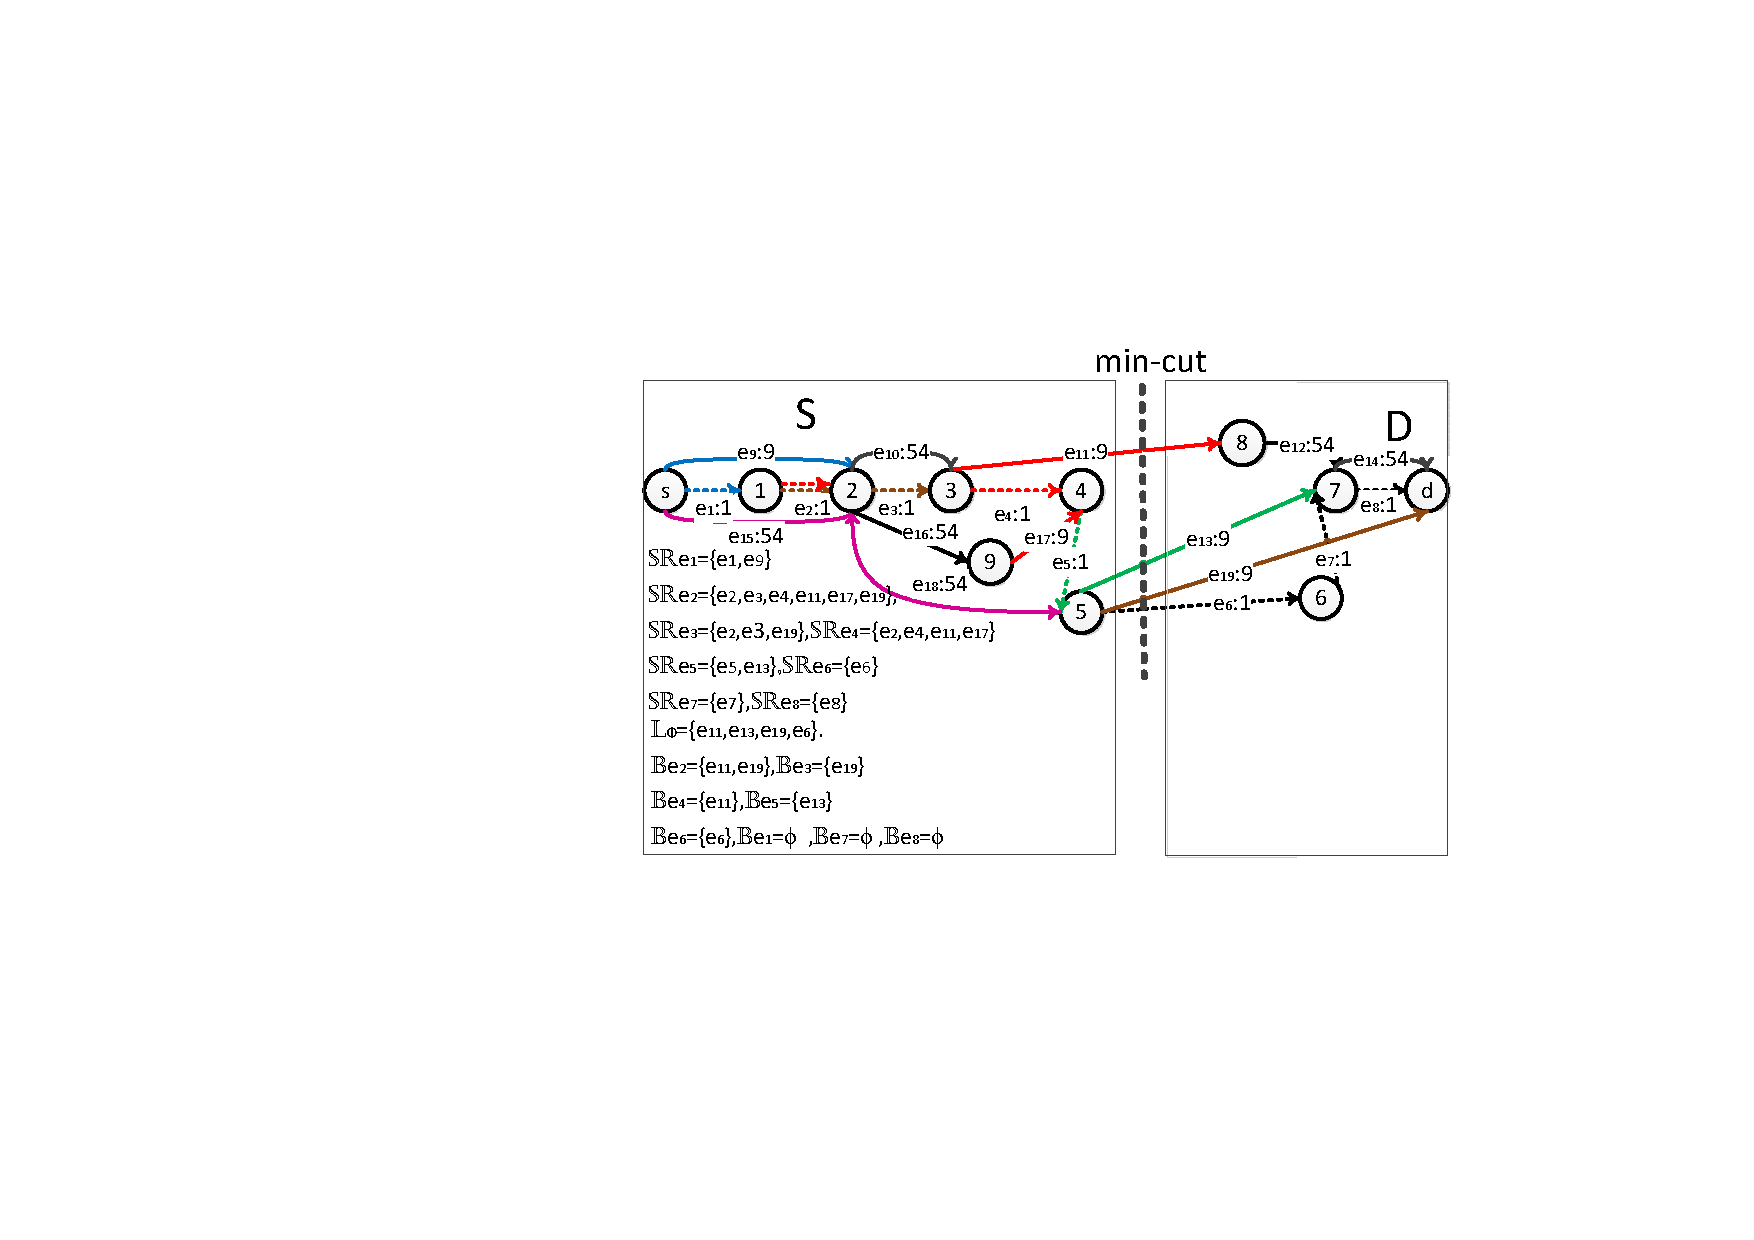
\includegraphics[width=4.5in]{figures/MinCutStarGraph}
  \caption{图$G^*$的最小割实例}\label{fig:MinCutStarGraph}
  \label{fig:MinCutStarGraph}
\end{figure*}

集合覆盖问题通常是一个NP-hard问题。它的复杂性取决于元素的大小(表示($N$)。 在提出的最小SRLG 冲突链路集问题中,$n=|\mathbb{L}_{\Phi}|$,即割集$\mathbb{L}_{\Phi}$ 的边数。因为本文的重点不是改进集合覆盖问题算法,应用\cite{chvatal1979greedy} 中提出的算法。在复杂度$O(log(|\mathbb{L}_{\Phi}|))$的情况下求出最小的SRLG 冲突链路集,通常即使是在大规模的网络,最短的路径作为AP都没有大跳数$n=|\mathbb{L}_{\Phi}|$。因此,用集合覆盖问题来求最小值SRLG冲突链路集代价不是很大。

为了说明如何找到最小SRLG冲突链路集,如图\ref{fig:MinCutStarGraph} 所展示了一个例子,求最小$\Phi(\mathbb{S},\mathbb{D})$, $\mathbb{S}=\{s, 1, 2, 3, 4, 5, 9\}$和$\mathbb{D}=\{d, 6, 7, 8\}$,边割集$\mathbb{L}_{\Phi}=\{e_{11},e_{13},e_{19},e_{6}\}$。对于AP路径上的所有链路,cut-block-link集合是:$\mathbb{B}_{e_1}=\emptyset$, $\mathbb{B}_{e_2}=\{e_{11},e_{19}\}$, $\mathbb{B}_{e_3}=\{e_{19}\}$, $\mathbb{B}_{e_4}=\{e_{11}\}$, $\mathbb{B}_{e_5}=\{e_{13}\}$, $\mathbb{B}_{e_6}=\{e_6\}$, $\mathbb{B}_{e_7}=\emptyset$ and $\mathbb{B}_{e_8}=\emptyset$。 为了覆盖$\mathbb{L}_{\Phi}$,最少的cut-block-link 集合是$\mathbb{B}_{e_2}=\{e_{11},e_{19}\}$,$\mathbb{B}_{e_5}=\{e_{13}\}$,$\mathbb{B}_{e_6}=\{e_6\}$。 因此,最小SRLG冲突链路集是$\mathbb{T}=\{e_2, e_5, e_6 \}$。

如图\ref{fig:MinCutStarGraph}所示的例子中,虽然$|\mathbb{L}_{\Phi}|=4$,但是最小SRLG冲突链路集$|\mathbb{T}|=|\{e_2, e_5, e_6 \}|=3$是小于$|\mathbb{L}_{\Phi}|=4$。这是因为$e_2$属于$\mathbb{R}_{r_2}$ 和$\mathbb{R}_{r_3}$,并能阻塞在割集$\mathbb{L}_{\Phi}$中的两条链路$e_{11}$ 和$e_{19}$


根据SRLG的拓扑类型\cite{datta2008graph},SRLG的拓扑类型:星型类型和非星型类型。对星型类型SRLG,所有链路都从同一个节点开始或结束在同一个节点。例如,如图\ref{fig:MinCutStarGraph}所示,$e_1$和$e_9$来自相同的节点$s$,$\mathbb{R}_{r_1}$是星型SRLG。对非星型类型,并不是SRLG 中的所有链路都是从相同节点开始或结束于同一节点。如图\ref{fig:MinCutStarGraph} 所示,$\mathbb{R}_{r_2}$, $\mathbb{R}_{r_3}$, $\mathbb{R}_{r_4}$ 和 $\mathbb{R}_{r_5}$是非星型类型。而且,即使在图\ref{fig:MinCutStarGraph} 所示包括星型SRLG 和无星型SRLG,提出的算法高效且有效地通过解决集合覆盖问题来解决冲突集。


因此,与现有的一些研究不同的是,文献\mycite{datta2008graph}只能处理单个SRLG 类型,这样的简单场景中一条链路只属于一个SRLG,提出的算法能更有效的处理多种情形。在更一般的情况下,链路可以属于一个或多个SRLG具有更多不同的SRLG 类型。
\subsection{算法步骤}
算法\ref{alg:min-min}显示了完整的min-min SRLG不相交路由算法。算法中的输入参数包括网络图($G$)、源节点($s$)、目的节点($d$)、包含链路集应包括在AP($\mathbb{I}$) 中,而排除链路集应不包含在AP($\mathbb{O}$)中。算法的输出结果是SRLG不相交路径对$(AP,BP)$。

为了寻找SRLG不相交路径,首先通过步骤\ref{alg:findap}中的FIND\_AP$(G,s,d, \mathbb{I},\mathbb{O})$搜索网络中最小权重AP路径,其中$\mathbb{I}=\phi,\mathbb{O}=\phi$,然后在步骤\ref{alg:findsrlgdisjointbp}中通过FIND\_SRLG\_Disjoint\_BP
$(G,s,d,AP)$搜索BP。特别是,可以通过Dijkstra 算法找到AP路径。为了计算BP,FIND\_SRLG\_Disjoint\_BP
$(G,s,d,AP)$包括两个步骤。首先,对于AP上的所有链路,删除与这些链路有共同风险的链路。第二,Dijkstra的算法再次运行在网络其余的链路上,计算从$s$到$d$的第二条最短路径BP。

如果能找到一个SRLG不相交的BP路径,则解决Min-Min SRLG不相交的路由问题,并如步骤\ref{alg:returnpathpair}所示返回找到的路径对。否则,就会出现陷阱问题。为了处理陷阱问题,步骤\ref{alg:findsrlgconflictinglinkset}首先找到SRLG冲突链路集$\mathbb{T}$,第\ref{alg:dividedandconquer} 步将原Min-Min SRLG 不相交路由问题划分为基于冲突集$\mathbb{T}$的$\left| \mathbb{T} \right|$个子问题。所有子问题都可以并行执行。步骤\ref{alg:findfeasible} 使用集合$\mathbb{F}$ 存储满足$A{P_i} \ne \phi$和$B{P_i} \ne \phi$的可行解。在$\mathbb{F}$中的所有可行解中,选择AP路径权重最低的路径对作为原Min-Min SRLG 不相交路由问题的最优解。

以图\ref{fig:CompositeGraph}中的例子来说明提出的算法\ref{alg:min-min}。根据步骤$\ref{alg:findap}$,提出的算法首先通过Dijkstra算法搜索路径权重最小的路径$\mathbb{AP}=\{e_1,e_2,e_3,e_4,e_5,e_6,e_7,e_8\}$,路径显示为图\ref{fig:CompositeGraph}(c)中的虚线。在删除AP上的链路以及与AP共享共同风险的链路之后,得到图\ref{fig:CompositeGraph}(d),这是一个不连通图没有BP路径。然而,如图\ref{fig:CompositeGraph}(b)所示,拓扑中实际存在一对SRLG不相交路径。因此,陷阱问题就会发生。在步骤$\ref{alg:findsrlgconflictinglinkset}$中找到SRLG冲突链路集$\{e_2,e_5,e_6\}$之后,采用分而治之的方法将原问题${\mathcal P}(\emptyset ,\emptyset )$划分为三个子问题,根据步骤$\ref{alg:findsrlgconflictinglinkset}$,并行执行这些子问题${\mathcal P}(\emptyset ,\{e_2\} )$, ${\mathcal P}(\{e_2\} ,\{e_5\} )$和${\mathcal P}(\{e_2,e_5\} ,\{e_6\} )$后,返回具有最小AP权重的路径对。


\begin{algorithm}[htb]
\caption{Min-Min SRLG不相交路径对算法}
\begin{algorithmic}[1]
\label{alg:min-min}
%\caption{Main process of Algorithm}
\REQUIRE
$G$: 网络图\\
$s$: 源节点\\
$d$: 目的节点 \\
$\mathbb{I}$:   必过链路集\\
$\mathbb{O}$: 必不过链路集\\
\ENSURE
AP: 主路径\\
BP: 备用路径
\STATE $AP=\emptyset$, $BP=\emptyset, \mathbb{I}=\emptyset, \mathbb{O}=\emptyset$
\STATE $AP\leftarrow$ FIND$\_$AP$(G,s,d,\mathbb{I},\mathbb{O})$\label{alg:findap}
\IF{$AP\neq\emptyset$}
    \RETURN $BP\leftarrow$ FIND\_SRLG\_Disjoint\_BP$(G,s,d,AP)$\label{alg:findsrlgdisjointbp}
    \IF{$BP\neq\emptyset$}
        \RETURN {路径对 $(AP,BP)$}\label{alg:returnpathpair}
    \ELSE
        \STATE 找到SRLG冲突链路集 $\mathbb{T}$\label{alg:findsrlgconflictinglinkset}
        \STATE $\mathbb{T}\leftarrow \mathbb{T}-(\mathbb{I}\cup\mathbb{O})$
        %\IF{$\mathbb{T}\neq \emptyset$}
        \STATE {分而治之的并行执行\\
        \small{
        $\!\!\!\!\!\!\!\!\!\!\!\!\!\!\!\!\!\!\!\left\{ \begin{array}{l}
 \left( {A{P_1},B{P_1}} \right)={{Min-Min}}\left( {G,s,d,\mathbb{I} ,\mathbb{O}\cup\{ {t_1}\} } \right), \\
 \left( {A{P_2},B{P_2}} \right)={{Min-Min}}\left( {G,s,d,\mathbb{I}\cup\{ {t_1}\} ,\mathbb{O}\cup\{ {t_2}\} } \right), \\
 \left( {A{P_3},B{P_3}} \right)={{Min-Min}}\left( {G,s,d,\mathbb{I}\cup\{ {t_1},{t_2}\} ,\mathbb{O}\cup\{ {t_3}\} } \right), \\
  \cdots  \\
 \left( {A{P_{\left| \mathbb{T} \right|}},B{P_{\left| \mathbb{T} \right|}}} \right) = {{Min-Min}}\left( {G,s,d,\mathbb{I}\cup \{ {t_1},{t_2}, \cdots ,{t_{\left| \mathbb{T} \right| - 1}}\} ,\mathbb{O}\cup\{ {t_{\left| \mathbb{T} \right|}}\} } \right) \\
 \end{array} \right.$
 }
        }\label{alg:dividedandconquer}
        \STATE{  {$\!\!\!\!\!\!\!\!\!\!\!F\leftarrow$ FIND\_FEASIBLE$(( {A{P_1},B{P_1}} )),\cdots,( {A{P_{|\mathbb{T} |}},B{P_{| \mathbb{T} |}}} )$}}\label{alg:findfeasible}
        %\ENDIF
         \IF{$F\neq{\emptyset,\emptyset}$}
         \RETURN{路径对 $(AP,BP)$ 满足条件 $AP = \mathop {\arg \min }\limits_{AP} \left\{ F \right\}$}
        \ENDIF

    \ENDIF
\ENDIF
\end{algorithmic}
\end{algorithm}

\subsection{算法时间复杂度}
\label{subsec:Complexity analysis}
当AP遇到陷阱问题时为了找到SRLG不相交路径对,我的算法首先计算出SRLG冲突链路集,然后通过把原问题划分成T个子问题来求解原问题。如\ref{subsec:Set cover problem for SRLG Conflicting Link Set}节所述边割集$\mathbb{L}_{\Phi}$ 的边数规模通常不是很大,因此,本算法寻找SRLG冲突链路集不会带来太多的时间成本。因此,关注的是路径查找过程的计算开销。

一般来说,对于一个有$|\mathbb{E}|$条链路和$|\mathbb{V}|$个节点的网络,求最小权重路径问题的时间复杂性是$(|\mathbb{E}|+|\mathbb{V}|)\times log(|\mathbb{V}|)$。为了解决陷阱问题,提出的路径查找问题与最初的最小权重路径问题有点不同。在路径查找的过程中引入了一些约束条件。例如,查找AP路径必须通过必过链路集$\mathbb{I}$和必不过链路集$\mathbb{O}$。由于这些链路集通常并不大,这些约束在成本计算上几乎没有差别。因为不同的子问题有不同的链路集,为了使描述简单明了,仍然使用$(|\mathbb{E}|+|\mathbb{V}|)\times log(|\mathbb{V}|)$ 作为一次路径搜索时间复杂度。而算法将原问题分成$|\mathbb{T}|$个子问题,算法复杂度为$|\mathbb{T}|\times(|\mathbb{E}|+|\mathbb{V}|)\times log(|\mathbb{V}|)$。


对于不同算法复杂性的比较,也展示了在CoSE\cite{rostami2007cose}和KSP\cite{eppstein1998finding}在路径查找过程中的复杂性。

CoSE试图找到一个冲突的SRLG集合,而不是一个冲突链路集。但是他们寻找冲突的SRLG集的方法是穷尽的查找而且成本很高。在这主要分析研究路径查找过程时间成本。由于提出的SRLG冲突链路集是由最小割和集合覆盖问题导出的,$|\mathbb{T}|$是最小的SRLG冲突链路集规模。因此,在CoSE中的冲突SRLG集至少是$|\mathbb{T}|$,并且表示SRLG集合为$\left\{ {SRL{G_1},SRL{G_2}, \cdots ,SRL{G_{|\mathbb{T}|}}} \right\}$,由于每个SRLG路径包含多条链路,因此CoSE的子问题应该比提出的要大得多。在AP路径上的一个SRLG 的必过链路集合和不过链路集会产生$|SRLG|$个子问题。所以一个SRLG集合$\left\{ {SRL{G_1},SRL{G_2}, \cdots ,SRL{G_{|\mathbb{T}|}}} \right\}$ 将引入$\prod\limits_{i = 1}^{_{\left| T \right|}} {\left| {SRL{G_i}} \right|}$个子问题。因此CoSE的复杂性$\prod\limits_{i = 1}^{_{|\mathbb{T}|}} {\left| {SRL{G_i}} \right|}\times (|\mathbb{E}|+|\mathbb{V}|)\times log(|\mathbb{V}|)$是比我提出的算法复杂度规模更大。

对于KSP算法\cite{eppstein1998finding},路径查找复杂度为$K\times ((|\mathbb{E}|+|\mathbb{V}|)\times log(|\mathbb{V}|))$,其中K是在发现SRLG不相交路径对之前应该测试的路径次数。然而,由于KSP没有从前面的路径搜索过程利用前面的信息,在最坏的情况下,KSP可能尝试从源节点$s$到目的节点$d$的所有路径。因此,最糟糕的K值是$2^{|\mathbb{E}|}$,这会带来很大的计算成本。

\section{实验配置与评价指标}
ubsection{实验配置}

因为找不到任何拓扑带有SRLG链路属性,所以通过注入SRLG信息生成一个合成的数据集。拓扑数据有$\TopoNum$种不同的拓扑,具有不同的节点数目、链路数目、链路权重,如表\ref{tab:AllSample}所示显示了拓扑的基本属性。这7 个拓扑中的节点、链路。

\begin{table*}[htbp]
\caption{SRLG拓扑数据}
  \centering
\footnotesize{  \begin{tabular}{*{18}{c}}
\toprule
拓扑 & 1 & 2 & 3 & 4 & 5 & 6& 7   \\
\midrule
点   &     527&      521    &      521     &    2023             &     451     &     521     &     449       \\
边   &    4158 &  4052     &    4152      &   4142          &       2780   &      4052   &      2778    \\
%Graph density  & 1.5\% &    1.49\% &   1.52\%  &  0.1\%  &   0.10\% &   1.41\%  &  1.5\% &   1.38\%   \\
No.SRLG & 132 &  86   &  89  &  207        & 210  &  128  &   88    \\
SRLG边比率 & 9.66\% & 6.16\% &   6.18\% &   14.94\%    &   22.55\%  &  9.65\% &   9.53\%     \\
\bottomrule
\end{tabular}
}
\label{tab:AllSample}
\end{table*}

为了进行性能比较,除了我提出的算法(\CI),还实现了另外四个SRLG完全不相交路径对算法。算法如下:
\begin{enumerate}
  \item ILP\cite{hu2003diverse}: 中的工作旨在寻找SRLG不相交路径对。通过整数线性规划方程使这两条路径总的权重最小化。没有找到其他通过整数线性规划方程寻找Min-Min SRLG不相交路径对的方法的研究。因此,从\cite{hu2003diverse} 的整数规划方程,通过改变目标函数构造Min-Min SRLG 不相交路径对问题的整数线性规划方程。
  \item IQCP\cite{hu2003diverse}:因为任意0−-1整数线性规划方程,其中所有变量为0或1,原问题的整数线性规划方程可以表示为一个二次约束方程,设计了Min-Min SRLG 不相交路径问题成一个整数二次约束规划(IQCP)\cite{hu2003diverse}。
  \item KSP\cite{eppstein1998finding}:它在源节点$s$和目的节点$d$中找到第K短路作为候选AP路径,一个接一个地测试候选的AP路径是否有相应的SRLG不相交路径BP,直到发现了这样的BP,算法才结束。
  \item CoSE\cite{rostami2007cose}:当AP遇到陷阱问题时,CoSE尝试进行简单而详尽的搜索,以找到一个SRLG集合。任何AP路径通过这个SRLG集都无法找到SRLG不相交的BP路径。基于这个SRLG集合,它划分原问题并设计算法来求SRLG不相交路径对。
\end{enumerate}

\subsection{评价指标}
ILP和IQCP是基于整数规划模型的。在提出的实现中,工具GUROBI 7.0\cite{optimization2012gurobi}用于解决这两个整数规划问题。六种性能指标用于评估不同的SRLG分路径算法:
\begin{itemize}
  \item 路径权重:路径中链路权重的总和。
  \item 路径跳数:路径中的跳数。
  \item 运行时间:查找SRLG不相交路径对的归一化平均时间。
  \item 算法加速比:给定两种不同的算法($alg_1$ 和$alg_2$)的计算时间,表示为$T_1$ 和 $T_2$,算法$alg_1$对于算法$alg_2$计算时间上的加速比是$alg_1$: ${S_{1 - 2}} = T_1/T_2$。
  \item 核加速比:并行程序的核心加速比\cite{grama2003introduction} 通常定义为$S_P=\frac{T_1}{T_p}$,其中p是处理器内核和$T_1$和$T_p$表示在1核和$p$核上的运行时间。
  \item 效率\cite{grama2003introduction}:定义为$E_p=\frac{S_p}{p}=\frac{T_1}{pT_p}$,它是百分比(0,1)的范围内。


\end{itemize}


所有实现都是在linux服务器上运行的,这个服务器配置Intel(R) Xeon(R) CPU E5-2620  2.00GHz 24 核和32.00GB内存。为了测量计算时间,在所有实现的算法中插入一个定时器。

通过在拓扑数据集里注入SRLG链路属性产生了两种SRLG类型,星型类型和非星型类型。在光纤网络中,SRLG是星型类型,而在其他网络类型中,例如一个Overlay网络中,SRLG 可以是非星型的。每个SRLG组是通过随机选择2-5链路组成的。在五种SRLG不相交路径对算法中,只有CoSE和SCLS是并行算法。尽管ILP、IQCP和KSP不是并行算法,仍然在实现它们来体现出我算法设计所获得的速度增益,平均化所有拓扑数据的结果为最终结果。


\subsection{算法性能评估及比较}
从节\ref{subsec:Complexity analysis}分析,在KSP下求第一条$K$最短路的计算复杂度是$2^{|\mathbb{E}|}\times ((|\mathbb{E}|+|\mathbb{V}|)\times log(|\mathbb{V}|))$,最坏的情况下这将是$K\times ((|\mathbb{E}|+|\mathbb{V}|)\times log(|\mathbb{V}|))$。与分析一致,当使用7个拓扑运行KSP,没有仿真结果能在1 小时内返回,而其他算法则可以在11 秒内。计算时间长使得KSP难以在实践中使用。因此,不在结果显示KSP。
\begin{enumerate}
  \item 路径权重:如图\ref{fig:normalization weitgh sum}所示,显示AP路径权重、BP路径权重和AP和BP的总和路径权重。显然,所有的算法SCLS、CoSE、ILP和IQCP 实现了相同的AP路径权重。但是不同的算法有不同的BP权重,因此它们有不同的路径权重和。因为所有算法都解决了SRLG不相交路径对问题,尽管他们发现不同的SRLG不相交路径对,它们都能达到找到最小权重相等的AP路径。然而,这两个基于整数线性规划的算法,ILP 和IQCP,主要是找到最小化AP的权重但是其随意找到其它任何SRLG不相交路径BP,因此这两个算法搜索到的BP路径是不同的。
  \item 路径跳数:图\ref{fig:normalization weitgh sum}显示AP路径跳数、BP 路径跳数和AP和BP路径跳数之和,因为所有算法的目标都是最小化SRLG不相交路径对的最小路径权重。如图\ref{fig:normalization weitgh sum} 所示在路径跳数中,它们具有相同的AP权重,但是如图\ref{fig:normalization hop} 所示他们有不同的AP 路径跳数。尽管所有算法的AP路径权重都小于BP 路径权重如图\ref{fig:normalization weitgh sum}所示,在图\ref{fig:normalization hop}中,AP跳数可能并不总是少于BP路径跳数。
  \item 运行时间:如图\ref{fig:normalization runtime}所示,通过改变使用的CPU核数来展示不同算法下的运行时间。由于CoSE下的运行时明显大于其他算法的运行时,为了更清楚地展示其他算法的结果,在图\ref{fig:Runtime_noKSP_noCOSE} 中通过排除CoSE来进一步绘制运行时间的结果。由于ILP和IQCP不是并行算法,这些算法在不同核数下的运行时间大致相等。提出的SCLS和CoSE的运行时间随着处理器核数的增加而减少,因为这两种算法可以将原问题划分为多个子问题来并行执行,并利用多核CPU的并行性来加快路径搜索的速度,虽然CoSE 是一种并行算法,但计算时间比ILP和IQCP 还要大。一些可能的原因包括:1)在CoSE中冲突SRLG集合的搜索过程效率不高;2)由于一个SRLG 通常包含多条链路,基于冲突SRLG问题的划分将带来大量的子问题需要解决,这也将带来大量的计算量。与CoSE不同的是,当AP上遇到陷阱问题时提出的SCLS根据图中的最小割集理论来求SRLG冲突链路集,并达到图\ref{fig:normalization runtime}中所示的最低时间消耗。这说明了提出的冲突链路集查找算法是有效的,并且提出的分治算法和基于SRLG冲突链路集的智能AP搜索过程,可以大大降低计算量。
   \item   算法加速比:如图\ref{fig:Multiple}所示,进一步比较了它们的计算速度。特别地,为了找出使用不同算法寻找所需路径时所获得的加速比,使用CoSE作为基准算法,并设置$alg_1$ =CoSE。与图\ref{fig:normalization runtime}中的结果相似,在图\ref{fig:Multiple} 中SCLS的加速度是CoSE的600倍以上。在图\ref{fig:Multiple} 中由于CoSE的运行速度明显小于其他算法,很难在图\ref{fig:Multiple}中观察到,在图\ref{fig:MultipleNoSCLS} 中排除了最大的SCLS 数据来进一步绘制了算法加速比结果。
   \item 核加速比:与使用算法加速比来比较所有算法的总体运行速度不同,这个度量“核加速比”是来评估CPU中的核数如何影响给定算法的运行速度。图\ref{fig:Speedup} 绘制了所有实现的算法的核加速比。算法ILP和IQCP下的核加速比在任意核数下近似等于1,因为它们不是并行算法。当核数小于4 时,提出的SCLS的核心加速比随着核数的增加而增加,当超过4核时,SCLS 的核心加速比保持稳定,说明4 核对SCLS是足够的。这一结果与Amdahl定律\cite{amdahl1967validity}是一致的,即理论核加速比确定的上界限定于问题的规模大小。但是,即使核心数等于8,CoSE下的核加速比也继续增加,这是数字4 的两倍。结果表明,即使是8核CPU也不能满足COSE的并行性要求.这是因为CoSE发现的冲突SRLG集包含了大量的链路,这进一步导致了大量的子问题,从而导致了较大的问题规模和计算成本。
    \item 效率:与图\ref{fig:Speedup}相似,随着更多的核增多效率值会降低,因为一个大的核心数会带来更多的成本来协调进程。如图\ref{fig:Efficiency}所示,所有算法的效率值都随着核心数的增加而降低。与图\ref{fig:Speedup}中的结果一致,由于CoSE 引入的子问题比提出的SCLS多,在核心数达到4之后,CoSE下的效率大于SCLS。然而,如图\ref{fig:Multiple}所示提出的SCLS实现了更大的算法加速比。
\end{enumerate}

全部仿真结果表明,在搜索速度较快的情况下,SCLS算法的性能优于其他算法,因为算法发现的冲突链路集可以方便有效的执行并行算法并且计算量小。

\begin{figure}[htb]
\centering
\begin{minipage}[t]{0.45\linewidth}
\centering
\includegraphics[width=2.25in]{figures/weight}
\caption{路径权重}
\label{fig:normalization weitgh sum}
\end{minipage}
\hfill
\begin{minipage}[t]{0.45\linewidth}
\centering
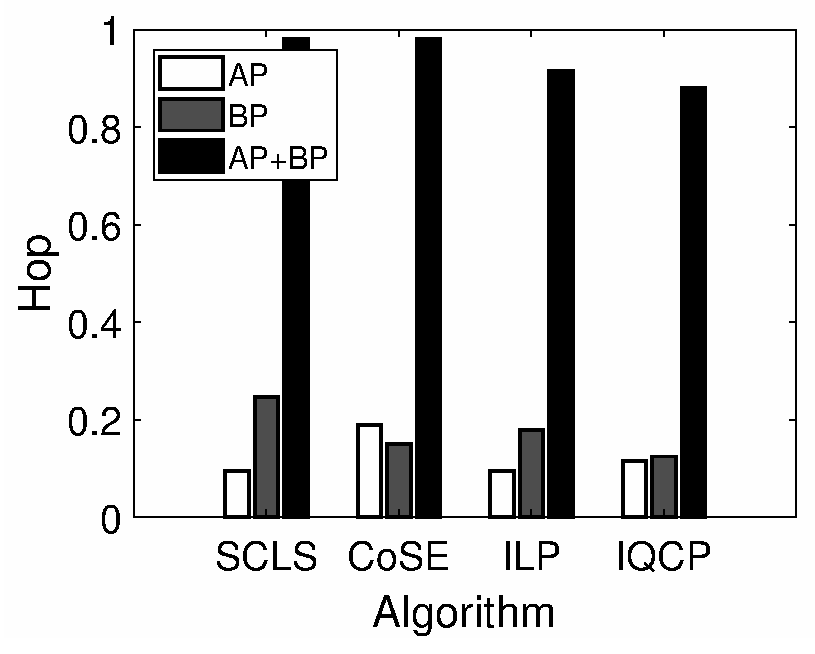
\includegraphics[width=2.25in]{figures/hop}
\caption{路径跳数}
\label{fig:normalization hop}
\end{minipage}
\end{figure}


\begin{figure*}[htb]
\centering
\begin{minipage}[t]{0.3\linewidth}
\centering
\includegraphics[width=2.25in]{figures/runtime}
\caption{运行时间}
\label{fig:normalization runtime}
\end{minipage}
\hfill
\begin{minipage}[t]{0.3\linewidth}
\centering
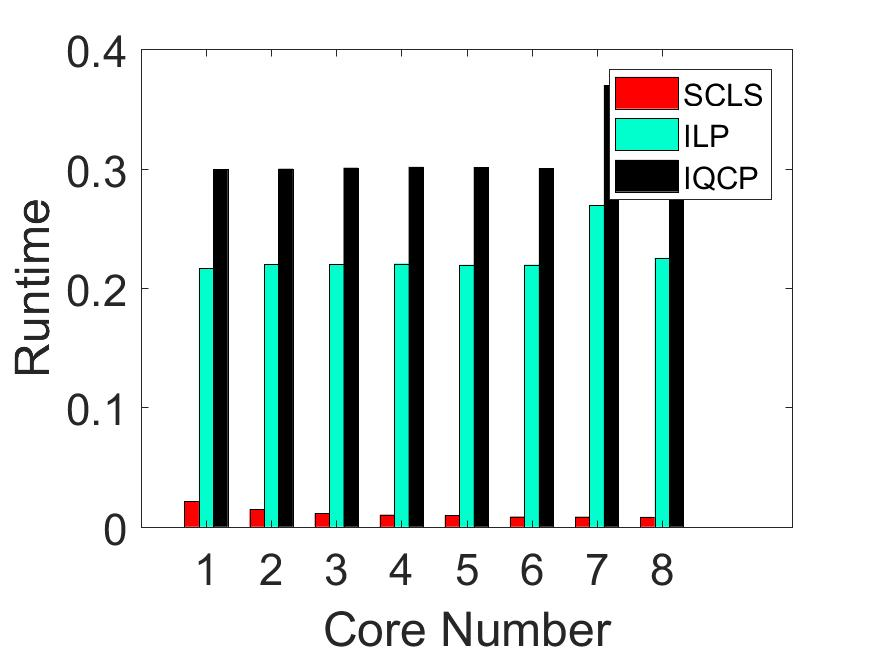
\includegraphics[width=2.25in]{figures/Runtime_noKSP_noCOSE}\\
  \caption{运行时间(无CoSE)}\label{fig:Runtime_noKSP_noCOSE}
\end{minipage}
\hfill
\begin{minipage}[t]{0.3\linewidth}
\centering
\includegraphics[width=2.25in]{figures/speedup}
\caption{核加速比}
\label{fig:Speedup}
\end{minipage}
\end{figure*}


\begin{figure*}[htb]
\centering
\begin{minipage}[t]{0.3\linewidth}
\centering
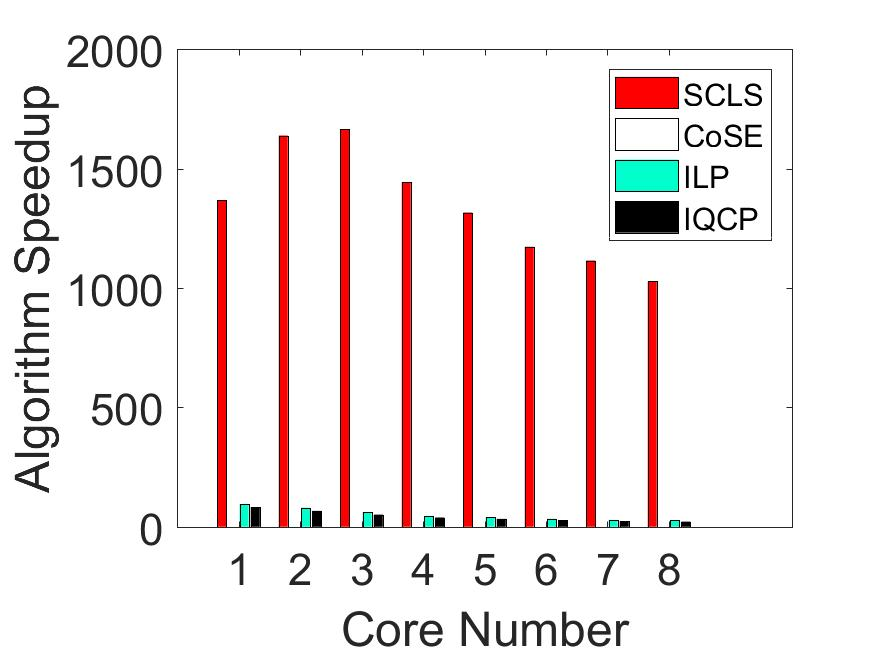
\includegraphics[width=2.25in]{figures/Multiple}
\caption{算法加速比}
\label{fig:Multiple}
\end{minipage}
\hfill
\begin{minipage}[t]{0.3\linewidth}
\centering
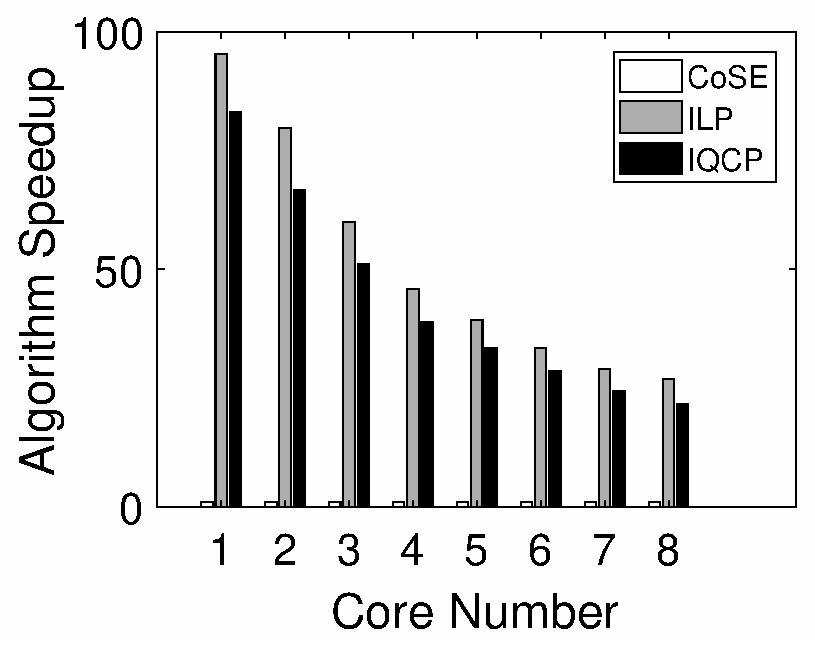
\includegraphics[width=2.25in]{figures/MultipleNoSCLS}
\caption{算法加速比(无SCLS)}
\label{fig:MultipleNoSCLS}
\end{minipage}
\hfill
\begin{minipage}[t]{0.3\linewidth}
\centering
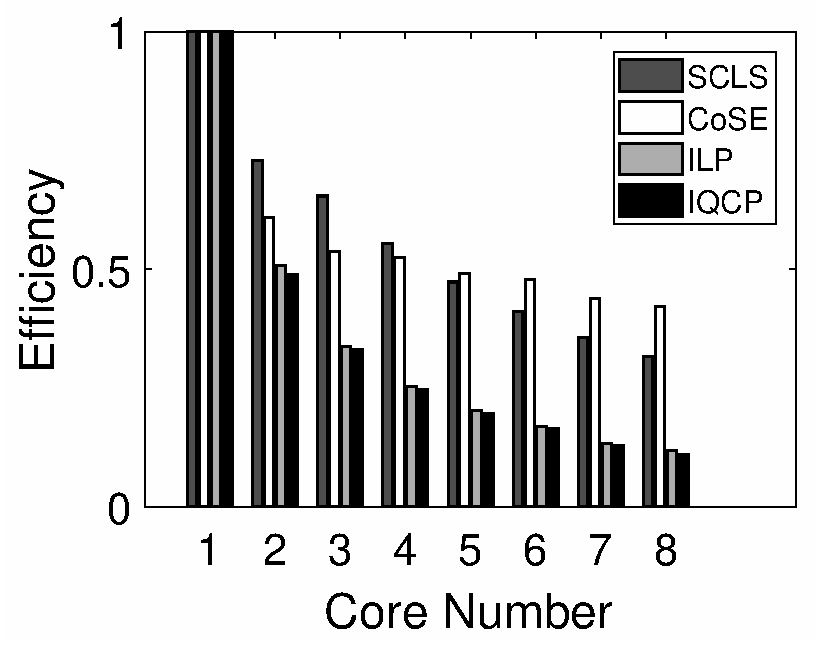
\includegraphics[width=2.25in]{figures/Efficiency}
 \caption{效率}
 \label{fig:Efficiency}
\end{minipage}
\end{figure*}
\section{小结}
本章提出了一种分而治之算法,该算法能在遇到陷阱问题时将原有的min-min SRLG 不相交路由问题划分为多个并行执行的子问题。与现有其它算法相比,提出的解决方案在搜索过程中利用现有的AP 搜索结果来加快求最优结果的速度,并且并行执行来进一步加快路径查找的速度。

